\documentclass[lettersize,journal]{IEEEtran}

\usepackage{amsmath,amsfonts,amssymb}
\usepackage{array}
\usepackage{stfloats}
\usepackage{url}
\usepackage{graphicx}
\usepackage{cite}
\newtheorem{theorem}{Theorem}
\newtheorem{proposition}{Proposition}
\newtheorem{corollary}{Corollary}
\newtheorem{lemma}{Lemma}
\newtheorem{remark}{Remark}
\hyphenation{op-tical net-works semi-conduc-tor IEEE-Xplore}
\def\BibTeX{{\rm B\kern-.05em{\sc i\kern-.025em b}\kern-.08em
    T\kern-.1667em\lower.7ex\hbox{E}\kern-.125emX}}

\urlstyle{same}
\begin{document}

\title{Multirobot Tracking of Separatrices and
Objective Eulerian Coherent Structures}

\author{Christopher Waight and Christopher A. Kitts,~\IEEEmembership{Senior Member,~IEEE}
\thanks{C. Waight is a PhD Candidate in the Robotic Systems Laboratory, Department of Mechanical Engineering, Santa Clara University, Santa Clara, CA 95053 USA (e-mail: cwaight@scu.edu)}
\thanks{C. A. Kitts is Professor and Director of the Robotic Systems Laboratory, Department of Mechanical Engineering, Santa Clara University, Santa Clara, CA 95053 USA (e-mail: ckitts@scu.edu)}
}
\markboth{IEEE Transactions on Robotics}%
{Waight and Kitts: Multirobot Tracking of Separatrices and Objective Eulerian Coherent Structures}

\maketitle

\begin{abstract}
Adaptive navigation is the process of modifying a robot's motion in
real time based on measurements taken while moving. This paper applies
that process to the boundaries that organize short-term transport in a
flow, the strain-dominated curves across which water masses separate
and along which floating material collects. Existing robotic trackers
of such structures either commit to the structure's identity before
tracking begins or accumulate an estimate over a finite integration
horizon. We present a cluster of six robots that does neither, using
only the instantaneous local flow measured simultaneously across the
formation. The cluster locates separating boundaries and holds station
on attracting ones. A cooperative estimator recovers the local quadratic field
model from one synchronous sample, six robots being the minimum for
the unconstrained model. The fit supplies two surrogates, the Jacobian
determinant, which traces separatrices but shifts under a rotating
observer, and the smaller rate-of-strain eigenvalue, which is
objective and recovers the identical material curve in any frame. We
develop an adaptive navigation primitive for each and characterize the
tradeoff between objectivity and noise tolerance. To our knowledge
this is the first demonstration of multirobot tracking of an objective
Eulerian coherent structure from instantaneous measurements alone. In a
rotating-frame trial the strain tracker holds the same material path
while the determinant tracker departs the structure; Monte Carlo
sweeps show the determinant tracker withstands about four to five
times more measurement noise, failing where the estimator gradient
stops being informative. Deployed on Santa Barbara Channel radar
currents, both primitives follow the same dominant transport corridor
for nearly the full record, separating only near landfall. The
controllers are admittedly simple, reactive, and minimal in robot
count; even so, they demonstrate acquisition, traversal, and terminal
capture on both analytic and measured fields, and yield an operational
rule for selecting between the two surrogates by field and mission.
\end{abstract}

\begin{IEEEkeywords}
Multirobot Systems, Adaptive Navigation, Coherent Structures,
Okubo-Weiss, Rate of Strain, Objectivity, Cooperative
Estimation, Cluster Space Control
\end{IEEEkeywords}

\section{Introduction}

\IEEEPARstart{I}{n} a coastal current, floating material does not
spread evenly, but rather collects along or separates across the
instantaneous coherent structures of the flow. Conventional survey
navigation finds these structures by covering the region with a
prescribed trajectory, whereas adaptive navigation (AN) does not,
instead modifying the vehicle's direction and motion path in real time
based on measurements taken while moving \cite{4}. These curves
come in two kinds: rotation-dominated cores, the eddies that retain
whatever enters them, and strain-dominated boundaries, the lines across
which neighboring water parcels are pulled apart. An oil sheen tracks
the attracting boundary and gathers on it within hours. A search object
caught on one side of a separating boundary does not cross to the other.
Knowing where these curves lie, and where they are going, is the difference
between searching a corridor and searching a basin.

Applying AN to coherent structures is challenging in current practice:
structure characterization is typically performed offline from a
reconstructed field, depends on an integration horizon that delays every
estimate, and requires an assumption about the structure's identity
before tracking begins.

AN in scalar fields is well developed and supplies the pattern. Each
robot contributes a single scalar measurement to a navigation policy
that reaches and follows a feature of interest, and each feature has
both a physical identity and an operational use. Maxima are hot spots
and pollutant sources; minima are sinks and marine anoxic zones;
contours bound the extent of a field or define a safety perimeter;
saddle points are low-energy passages; ridges are resource divides and
paths of maximum service availability on departure; trenches are
accumulators and paths of minimum exposure on approach
\cite{2,3,4,5}. Formations are sized so that differential measurements
across the cluster recover the gradient and curvature each policy
consumes \cite{2,6}.

Vector fields, which assign both a magnitude and a direction to each
point, carry their own catalog of features, and the same mapping from
mathematics to mission applies. Critical points are the isolated
members. Sinks are convergence zones and areas of high probability
for search and rescue \cite{7}; sources are divergences where spewing
fluid points to a below-surface leak \cite{8}; eddy centers are
retained water masses and station-keeping points for persistent
observation. In \cite{9}, a
three-robot cluster estimated the location and type of an isolated
critical point from a linear fit of simultaneous local velocity
measurements, recovering the feature from instantaneous data alone.

The extended features are the subject of this paper. A separatrix is a
transport barrier and a containment boundary, the curve a pollutant
plume will not cross and the line along which a coastal sensor array is
best deployed \cite{13,14,15}. Its saddle points are the stagnation
points of the flow, the junctions where two such barriers cross and
where the corridor a drifter follows is decided. An attracting
objective Eulerian coherent structure (OECS) is a convergence line and
an accumulator, the curve on which floating debris, larvae, and search
objects collect, and therefore the curve a search pattern should
follow rather than cross \cite{35}. Fronts, the dynamically meaningful
lines along which water masses converge, are the scalar-field
counterpart, and coordinated multi-vehicle sampling of such dynamic
ocean features is itself an active area of marine robotics, spanning
drifter-referenced AUV surveys \cite{10}, front-tracking ASV/AUV teams
\cite{11}, and adaptive glider fleets \cite{12}. Like the related
Okubo-Weiss field used to classify oceanic mesoscale eddies \cite{16},
these structures can in principle be inferred from instantaneous
measurements alone, which is what makes them candidates for AN.

Multirobot systems are the appropriate platform for this class of
problem on sensing grounds. A single vehicle must move laterally to
sense a local gradient, which costs time and is detrimental in a
time-varying field, whereas a cluster shares simultaneously collected,
spatially distributed measurements, additionally accommodates vehicle
failures, and adapts its formation size and shape to the spatial
frequencies present in the field \cite{3,4}. The third of these is a
specifiable mission attribute: the operator may select the cluster
size, trading spatial resolution, differential signal amplification,
noise suppression, and breadth of field exploration against one
another for a given number of robots \cite{6}. These systems now
operate across land, sea, air, and space \cite{1}.

Our own prior work in this field has matured from scalar-field
primitives \cite{3,4,5} through isolated vector-field critical points
\cite{9} to the extended structures treated here. This work presents
results of that continuing program. Our current focus is the pair of
surrogates below and the operational rule for choosing between them.

This paper contributes a) a cooperative second-order estimator that
recovers the local quadratic model of a two-component field from one
synchronous sample, with six robots proved minimal, a conic
characterization of the formations that fail, and exact,
heading-isotropic noise gains; b) two AN primitives, the $D$ tracker
and the $s_1$ tracker, that read the two terms of one splitting
identity, $D = \omega^2/4 - s_1^2$, off the same six-robot fit;
c) closed-loop frame equivariance of the $s_1$ tracker, demonstrated
in a rotating-frame trial against the $D$ tracker's demonstrated
departure under the same rotation; and d) a characterized tradeoff
between that objectivity and noise tolerance, diagnosed down to a
specific estimator channel, together with a selection rule for
choosing between the two primitives by field and mission. Both
primitives are exercised on real Santa Barbara Channel radar currents.

The remainder of the paper reviews related work, formulates the
problem (Section~\ref{sec:detj_field}), develops the estimator
(Section~\ref{sec:estimation}) and the two primitives
(Section~\ref{sec:controllers}), and reports the simulation program
and its results (Section~\ref{sec:results}).

\subsection{Related Work}
\label{sec:related_robots}

Haller and Yuan formalized the Lagrangian coherent structure (LCS) as
the generalization of stable and unstable manifolds to flows with
arbitrary time dependence \cite{13}. The standard computable
definition, a ridge of the finite-time Lyapunov exponent (FTLE) field,
is given in \cite{15} on the same double-gyre model used throughout
this paper. The objectivity and Lagrangian/Eulerian tradeoff that
bears on any Eulerian surrogate is developed in \cite{23,24,25}.
Velocity-gradient recovery from sparse trajectories \cite{26} and the
strain-spin decomposition itself \cite{27} remain active adjacent
directions. The instantaneous criteria remain the computable
workhorses. Okubo and Weiss partition a planar flow from the local
velocity gradient alone \cite{28,29}, generalized to three dimensions
\cite{30}, refined for oceanographic use \cite{31}, and used at scale
in mesoscale eddy censuses \cite{16}.

The nearest prior work tracks a coherent structure directly with a
robot formation. Michini et al. bracket a presumed stable or unstable
manifold with three robots using only local velocity measurements
\cite{17}, verified in simulation and in a laboratory flow tank with
micro surface vehicles, and evaluated against a measured Santa Barbara
Channel radar record. The strategy extends to $N$ robots \cite{18} and
was validated on the same class of vehicles \cite{19}. Its robots
begin on the manifold and are advected by the flow, the manifold's
identity is supplied before tracking begins, and the saddle point is
not treated by either the controller or its analysis; \cite{17}
reports veering away from the structure near a saddle, where the flow
reverses on the far side, in both its flow-tank and its ocean trials.
Kularatne and Hsieh instead compute the local FTLE field on board,
which recovers the structure's type at the cost of a nonzero
integration horizon, verified in simulation \cite{21}. Unlike methods
that sense only a scalar reduction of the field \cite{32}, the cluster
here fits the full local quadratic vector field, so the surrogate's
shape, not merely its sign, is available to the primitives, and the
curvature of the field itself is estimated rather than assumed, which
is what fixes not just where a structure lies but what kind it is and
how many branches meet there.

On the estimation side, \"{O}gren, Fiorelli, and Leonard established
cooperative gradient climbing with a formation of mobile sensors
\cite{2}, and Bri\~{n}\'{o}n-Arranz, Renzaglia, and Schenato extended
the idea to the Hessian, with five robots on a ring plus one at the
center recovering the gradient and Hessian of a scalar signal in
closed form \cite{6}. McDonald, Kitts, and Neumann developed the
complementary AN primitives that follow scalar-field ridges, trenches,
and saddle points from local differential measurements alone
\cite{3,4,5}. Each of these formations samples a single signal
channel. A coupled two-component field doubles the estimation problem
to twelve unknowns, and \cite{6}'s fixed symmetric weights hold for
the ideal ring geometry, where the estimator here solves at the
measured positions and stays exact as the formation deforms.

This paper and the critical-point and structure-tracking methods above
\cite{9,17,18,19,20,21} navigate a naturally occurring flow sensed in
situ, unlike the separate literature that builds an artificial vector
field as a synthetic guidance signal for single-robot path following
\cite{33} or obstacle avoidance \cite{34}.

\section{Problem Formulation}
\label{sec:detj_field}

\subsection{Vector Fields and Local Polynomial Models}

A planar vector field assigns a velocity vector $\mathbf{v}(\mathbf{p}) =
(u(\mathbf{p}), v(\mathbf{p}))$ to each position $\mathbf{p} = (x, y)$ in its
domain. The critical-point estimator of \cite{9} fits a \emph{planar}
(affine) model of each component to simultaneous measurements and solves
the linear system for the point where $\mathbf{v} = \mathbf{0}$. The
surrogates this paper tracks are built not from $\mathbf{v}$ but from its
spatial derivatives, and navigating them requires derivatives through
second order. A planar fit, whose second derivatives are identically zero,
cannot supply them.

The cluster therefore works from the second-order Taylor expansion of
each component about the cluster centroid $\mathbf{p}_c$. Coordinates
$\mathbf{p} = (x, y)$ are measured from the centroid throughout this
section, so that $\mathbf{p} = \mathbf{0}$ is the centroid itself.
\begin{align}
    u(\mathbf{p}) &= a_1 + a_2 x + a_3 y
        \nonumber \\
        &\quad + a_4 xy + \tfrac{1}{2} a_5 x^2 + \tfrac{1}{2} a_6 y^2
        + \mathcal{O}(\|\mathbf{p}\|^3),
        \label{eq:quad_model_u} \\
    v(\mathbf{p}) &= b_1 + b_2 x + b_3 y
        \nonumber \\
        &\quad + b_4 xy + \tfrac{1}{2} b_5 x^2 + \tfrac{1}{2} b_6 y^2
        + \mathcal{O}(\|\mathbf{p}\|^3).
        \label{eq:quad_model_v}
\end{align}
The twelve coefficients are constants, and all position dependence is
carried by $x$ and $y$. Each coefficient is a derivative of the field at
the centroid, the one-half factors chosen so that the match is direct,
giving $a_1 = u(\mathbf{p}_c)$, $a_2 = \partial u/\partial
x|_{\mathbf{p}_c}$, $a_4 = \partial^2 u/\partial x \partial
y|_{\mathbf{p}_c}$, $a_5 = \partial^2 u/\partial x^2|_{\mathbf{p}_c}$,
and likewise for $b_1, \ldots, b_6$ with $v$ in place of $u$. Where a
partial derivative of the true field is meant rather than a fitted
coefficient, this paper writes it as a derivative, $u_x$, $u_{xy}$, and
so on.

The cluster estimates these coefficients by fitting the quadratic model
that remains when the $\mathcal{O}(\|\mathbf{p}\|^3)$ remainder is
discarded, and marks the results with a hat. $\hat{a}_5$ is an estimate
of $a_5$, not the quantity itself. Two mechanisms separate them. Sensor
noise perturbs each measurement, and truncation bias arises because the
discarded cubic terms are not zero over a footprint of finite size, so
the fit absorbs part of them into the retained coefficients.

The first-order coefficients are the centroid values of the entries of the
field Jacobian
\begin{equation}
    \mathbf{J}(\mathbf{p}) =
    \begin{bmatrix}
        \partial u / \partial x & \partial u / \partial y \\
        \partial v / \partial x & \partial v / \partial y
    \end{bmatrix},
\end{equation}
so that $\mathbf{J}_0 = \mathbf{J}(\mathbf{p}_c)$ has entries $a_2$,
$a_3$, $b_2$, $b_3$, and we write $D(\mathbf{p}) =
\det(\mathbf{J}(\mathbf{p}))$ throughout.

\subsection{The Determinant Surrogate $D$}

The Okubo-Weiss parameter \cite{28,29}, built from the normal strain,
shear strain, and vorticity
($\omega = \partial v/\partial x - \partial u/\partial y$), satisfies
$Q = \tfrac{1}{4}(\nabla \cdot \mathbf{v})^2 - D$ by direct expansion
under the quarter-normalized convention of \cite{31}; the common
unhalved-strain convention $Q = s_n^2 + s_s^2 - \omega^2$ instead gives
$Q = -4D$ for incompressible flow. For the incompressible flows
considered here $Q \propto D$ exactly either way, so we
work with $D$. The sign of $D$ fixes the local eigenstructure.
Incompressibility gives $\operatorname{tr}(\mathbf{J}) = 0$, so the
eigenvalues $\mu_J$ of $\mathbf{J}$ satisfy
\begin{equation}
    \mu_J = \pm\sqrt{-D} \ \ (D < 0), \qquad
    \mu_J = \pm i\sqrt{D} \ \ (D > 0).
\end{equation}
Where $D < 0$ the flow is locally hyperbolic (strain-dominated) and
nearby particles separate at the instantaneous exponential rate
$\sqrt{-D}$, the frozen-time linearization's eigenvalue rate rather than
the material stretching rate; the two coincide only where $\omega = 0$,
since the material rate is $s_2 = -s_1$.
Where $D > 0$ it is locally elliptic (rotation-dominated),
and the zero level set of $D$ is the Okubo-Weiss boundary between the
two regimes. The more negative $D$ is, the stronger the local
hyperbolicity, so trenches (valley lines) of $D$ inside strain regions
mark the loci of strongest instantaneous attraction and repulsion.

\subsection{The Strain-Eigenvalue Surrogate $s_1$}
\label{sec:strain_field}

The Cauchy--Stokes decomposition splits the velocity gradient into
symmetric and antisymmetric
parts, $\mathbf{J} = \mathbf{S} + \mathbf{W}$, with rate-of-strain
tensor $\mathbf{S} = (\mathbf{J} + \mathbf{J}^\top)/2$ and spin tensor
$\mathbf{W} = (\mathbf{J} - \mathbf{J}^\top)/2$, which carries the
vorticity. Consider a time-dependent change of observer
$\mathbf{p}' = \mathbf{Q}(t)\mathbf{p} + \mathbf{b}(t)$, with rotating
frame $\mathbf{Q}(t)$. For the special case
$\mathbf{p}' = \mathbf{Q}(t)\mathbf{p}$, the convention used in the
rotating-frame trial of this paper, write
$\dot{\mathbf{Q}}\mathbf{Q}^\top = \Omega\left[\begin{smallmatrix} 0 &
-1 \\ 1 & 0 \end{smallmatrix}\right]$, so $\Omega$ is the frame's own
angular rate. The frame's rotation enters the velocity gradient only
through this antisymmetric term, so it lands entirely in the spin
part, $\omega' = \omega + 2\Omega$, while the strain part transforms
cleanly, $\mathbf{S}' = \mathbf{Q}\mathbf{S}\mathbf{Q}^\top$. The
eigenvalues $s_1 \leq s_2$ of $\mathbf{S}$ are therefore
frame-invariant, its eigenvectors $\mathbf{e}_1, \mathbf{e}_2$
co-rotate with the frame, and quantities built from them are
objective. Material behavior, which cannot depend on the observer, can
be predicted from them in any frame \cite{23,24}.

For any symmetric $\mathbf{S}$ and antisymmetric $\mathbf{W}$ the cross
term vanishes, $\operatorname{tr}(\mathbf{S}\mathbf{W}) = 0$, so the
determinant splits exactly.
\begin{equation}
    D \;=\; \det\mathbf{S} + \det\mathbf{W}
      \;=\; s_1 s_2 + \frac{\omega^2}{4}
      \;=\; \frac{\omega^2}{4} - s_1^2,
    \label{eq:splitting}
\end{equation}
the middle equality holding generally, and the last specializing to
incompressible flow ($s_2 = -s_1$). Four consequences of
(\ref{eq:splitting}) organize everything that follows.
First, the Okubo-Weiss partition is the competition between the two
terms, rotation-dominated where the spin term wins ($D > 0$),
strain-dominated where the strain term wins ($D < 0$). Second,
substituting $\omega' = \omega + 2\Omega$ gives
\begin{equation}
    D' = D + \Omega\,\omega + \Omega^2,
    \label{eq:D_not_objective}
\end{equation}
so two observers rotating relative to one another disagree about where
the $D$ structures are. The frame artifact lives entirely in the spin
term, so every quantity derived from $D$ inherits it and every quantity
derived from $s_1$ carries none.
Third, where the vorticity vanishes the identity collapses to
$s_1 = -\sqrt{-D}$. The two surrogates coincide on vorticity-free
lines and part ways everywhere else. Fourth, differentiating
(\ref{eq:splitting}) transverse to a curve gives
\begin{equation}
    \frac{\partial D}{\partial n} =
    \frac{\omega}{2}\frac{\partial \omega}{\partial n}
    - 2 s_1 \frac{\partial s_1}{\partial n},
    \label{eq:trench_coincide}
\end{equation}
so on a curve where the vorticity vanishes and the flow is
strain-dominated ($s_1 < 0$), the two transverse derivatives vanish
together and the two trenches are not merely coincident but tangent to
the same curve.

The smaller eigenvalue $s_1$ is the local instantaneous contraction
rate. Where $s_1 < 0$, material filaments are compressed along
$\mathbf{e}_1$ and stretched along $\mathbf{e}_2$ at rate $s_2 = -s_1$.
An attracting OECS is a trench of the signed scalar field $s_1$ ridden
along the stretching eigenvector $\mathbf{e}_2$, a curve on which
$s_1 < 0$ is locally most negative in the transverse direction, so
neighboring material is drawn onto it \cite{24}. This is the objective
counterpart of the $D$ trench. Serra et al. extracted these structures
from instantaneous surface-current measurements and confirmed in field
trials at sea that floating objects collect onto them within hours
\cite{35}.

One caution accompanies the eigenstructure. $\mathbf{e}_1,
\mathbf{e}_2$ are direction fields with no globally consistent sign,
undefined at isotropic points of $\mathbf{S}$ ($s_1 = s_2$), so the
primitive must orient its tangent by continuity rather than by any
pointwise rule.

\subsection{The Double-Gyre Example}
\label{sec:dg_example}

The double-gyre flow used throughout is the steady ($\varepsilon = 0$)
member of the Shadden family \cite{15}, shifted from the canonical domain
$[0,2] \times [0,1]$ to $[-1,1] \times [-0.5, 0.5]$ by
$x_f = x + 1$, $y_f = y + 0.5$, where $(x_f, y_f)$ are field-frame and
$(x, y)$ world-frame coordinates. Both are non-dimensional throughout the
double-gyre experiments, so distances and gaps reported in world-frame
units carry no further unit conversion unless stated. The field is
\begin{equation}
    u = -\pi A \sin(\pi x_f) \cos(\pi y_f), \quad
    v = \pi A \cos(\pi x_f) \sin(\pi y_f),
    \label{eq:dg_u}
\end{equation}
with $A = 0.1$. The flow is incompressible, the separatrix is the line
$x = 0$, the saddle points are $\mathbf{p}^*_1 = (0, -0.5)$ and
$\mathbf{p}^*_2 = (0, 0.5)$, and the gyre centers are $(\pm 0.5, 0)$.
The unsteady member of the same family, used once in
Section~\ref{sec:disc_clean} as a spot check, replaces $x_f$ in
(\ref{eq:dg_u}) with
\begin{equation}
    \tilde{x}_f = \varepsilon \sin(\omega_{dg} t)\,x_f^2
        + \bigl(1 - 2\varepsilon\sin(\omega_{dg} t)\bigr)\,x_f ,
    \label{eq:dg_unsteady}
\end{equation}
so that the separatrix oscillates about $x = 0$ with amplitude set by
$\varepsilon$ and angular frequency $\omega_{dg}$, recovering the steady
field at $\varepsilon = 0$.

All quantities of interest have closed forms. The Jacobian entries are
$u_x = -\pi^2 A \cos\pi x_f \cos\pi y_f = -v_y$ and
$u_y = \pi^2 A \sin\pi x_f \sin\pi y_f = -v_x$, so the flow is divergence
free, and direct differentiation of (\ref{eq:dg_u}) with the double-angle
identities gives
\begin{equation}
    D(\mathbf{p}) = -\frac{\pi^4 A^2}{2}
    \bigl(\cos 2\pi x_f + \cos 2\pi y_f\bigr),
    \label{eq:det_analytic_main}
\end{equation}
\begin{equation}
    \begin{aligned}
    \nabla D &= \pi^5 A^2
    \begin{bmatrix} \sin 2\pi x_f \\ \sin 2\pi y_f \end{bmatrix},
    \\
    \mathbf{H}_D &= 2\pi^6 A^2
    \begin{bmatrix} \cos 2\pi x_f & 0 \\ 0 & \cos 2\pi y_f \end{bmatrix},
    \end{aligned}
    \label{eq:gradhess_analytic_main}
\end{equation}
with vorticity $\omega = -2\pi^2 A \sin\pi x_f \sin\pi y_f$. Three facts
follow directly. First, the Okubo-Weiss boundary is the diamond
$x_f \pm y_f \in \tfrac{1}{2} + \mathbb{Z}$ inscribed around each gyre
center, $D > 0$ inside.

Second, the separatrix is a trench of $D$. Cross-track curvature
$2\pi^6 A^2 > 0$ on $x = 0$ (Fig.~\ref{fig:trench_cross}), deepest at
the two saddles, rising to a crest ($D = 0$, vorticity also zero, so
$\sqrt{-D}$ by (\ref{eq:splitting}) is the attraction rate toward it)
at the origin, where a descend-only primitive stalls. Periodicity
turns the trenches of $D$ into a grid whose right-angle crossings
are the saddle points, so a tracker continuing past a saddle is still
on a trench.

Third, the strain field shares the grid but signs its segments. The
shear strain vanishes identically, so $\mathbf{S} =
\mathrm{diag}(u_x, -u_x)$ everywhere, eigenvectors fixed on the
coordinate axes away from the degeneracy lines
$\cos\pi x_f \cos\pi y_f = 0$, giving
\begin{equation}
    s_1 = -\pi^2 A\,\lvert\cos \pi x_f \cos \pi y_f\rvert,
    \label{eq:s1_analytic_main}
\end{equation}
with the trench minima $s_1 = -\pi^2 A$ at the six flow saddles, the
terminal cores a traverse settles at, the two separatrix saddles
$\mathbf{p}^*_1$, $\mathbf{p}^*_2$ and, by the periodicity of
(\ref{eq:det_analytic_main}), the four further crossings the domain
walls carry at $x = \pm 1$, $y = \pm 0.5$.
Equation~(\ref{eq:s1_analytic_main}) shows $s_1$ is a transverse trench
of the separatrix on \emph{both} halves, with no sign change and no
ridge to cross. What alternates by segment is the \emph{material}
identity of its tangent, the stretching eigenvector $\mathbf{e}_2$ above
and the compression eigenvector $\mathbf{e}_1$ below, swapping at the
origin, the isotropic point of $\mathbf{S}$ where the $D$ crest sits
and $\mathbf{e}_1, \mathbf{e}_2$ are simultaneously undefined. By the
definition of Section~\ref{sec:strain_field} the upper segment is an
attracting OECS and the lower a repelling one, joined at that point. An
objective tracker that keys its transverse channel to the trench of
$s_1$ rather than to a named eigenvector needs no ridge detector and no
special handling at the isotropic point.

\begin{figure}[!t]
    \centering
    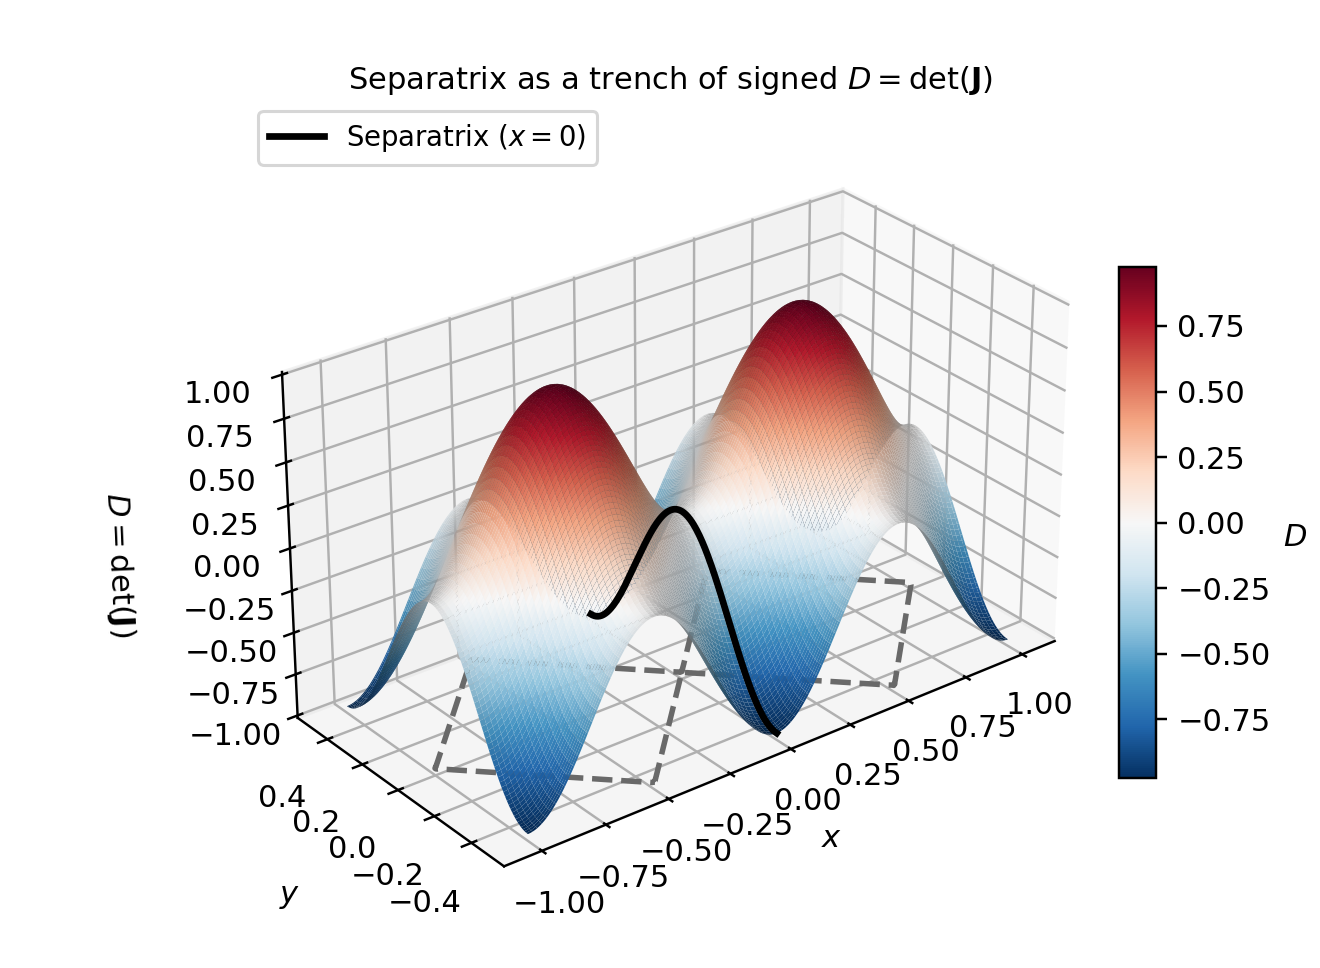
\includegraphics[width=0.40\textwidth]{figures/detJ_trench_cross_section.png}
    \caption{Signed $D$ as an elevation surface over the double gyre.
    The gyre cores rise as ridges ($D > 0$). The separatrix at $x = 0$
    (bold) is a trench of $D$, deepest at the saddles and rising to
    $D = 0$ at the origin.}
    \label{fig:trench_cross}
\end{figure}

\subsection{Problem Statement}
\label{sec:problem_statement}

Consider six robots at positions $\mathbf{p}_i$, the minimum cluster
Proposition~\ref{prop:minimality} establishes for this recovery, each
measuring the local flow $(u_i, v_i) = \mathbf{v}(\mathbf{p}_i)$ at the
common sampling instant, with no map, forecast, or prior field model and
no trajectory integration. The measured flow is a sampled datum, not a
current that advects the platform. Robot motion is commanded by the
control law, not advected by the sampled flow. Using only the current
synchronous samples at each control cycle, the cluster must generate a
centroid velocity command $\dot{\mathbf{p}}_c$ that solves one of two
problems, one per term of (\ref{eq:splitting}).

\emph{Problem 1 (separatrix network traversal).} Drive the cluster
centroid onto the trench of $D$ and travel it, in the direction of the
ambient flow, through the saddle points where trench segments cross.

\emph{Problem 2 (objective network traversal).} Drive the centroid onto
the trench of $s_1$ and travel it, in the direction the ambient flow
sets at first contact, through the isotropic point where the
attracting and repelling OECS meet, and detect and hold at a terminal
attracting core where one is reachable, using objective quantities
throughout apart from that one-time seed.

\section{Cooperative Second-Order Estimation}
\label{sec:estimation}

\subsection{Quadratic Fit from Six Simultaneous Measurements}

With robot positions $\mathbf{p}_i = (x_i, y_i)$ again measured from the
centroid, define the quadratic basis vector
\begin{equation}
    \boldsymbol{\phi}(\mathbf{p}) =
    \bigl[\,1, \; x, \; y, \; xy, \;
    \tfrac{1}{2}x^2, \; \tfrac{1}{2}y^2\,\bigr]^\top,
\end{equation}
whose entries are the terms of
(\ref{eq:quad_model_u})--(\ref{eq:quad_model_v}) in the same order, so
the recovered coefficients estimate the Taylor derivatives directly with
no rescaling. Stacking the six robots' basis vectors row-wise gives
the $6 \times 6$ formation matrix $\boldsymbol{\Phi}$, and the coefficient
estimates $\hat{\boldsymbol{\theta}}_u = [\hat{a}_1, \ldots,
\hat{a}_6]^\top$ and $\hat{\boldsymbol{\theta}}_v = [\hat{b}_1, \ldots,
\hat{b}_6]^\top$ solve
\begin{equation}
    \boldsymbol{\Phi}\,\hat{\boldsymbol{\theta}}_u = \mathbf{m}_u, \qquad
    \boldsymbol{\Phi}\,\hat{\boldsymbol{\theta}}_v = \mathbf{m}_v,
    \label{eq:solve}
\end{equation}
where $\mathbf{m}_u = [u_1, \ldots, u_6]^\top$ and
$\mathbf{m}_v = [v_1, \ldots, v_6]^\top$ collect the measurements, $u_i$
and $v_i$ being the field components sampled by robot $i$. One matrix
factorization serves both components. If the field is exactly quadratic
over the formation footprint, the $\mathcal{O}(\|\mathbf{p}\|^3)$
remainder vanishes identically, and noise-free measurements give
$\hat{\boldsymbol{\theta}}_u = \boldsymbol{\theta}_u$ and
$\hat{\boldsymbol{\theta}}_v = \boldsymbol{\theta}_v$ for any nonsingular
$\boldsymbol{\Phi}$. Neither condition holds exactly in practice.

\begin{proposition}[Minimality]
\label{prop:minimality}
A synchronous sample from fewer than six robots leaves the
unconstrained quadratic model unidentifiable.
\end{proposition}

\begin{IEEEproof}
Each robot contributes one equation per component to (\ref{eq:solve}),
and each system has six unknowns, so fewer than six robots leave the
solution set a positive-dimensional affine subspace.
\end{IEEEproof}

Any method returning a single answer from five robots is therefore
supplying a structural prior rather than reading one from the data. Such
a prior is available. Imposing exact incompressibility ties $a_2 + b_3 =
0$ together with its two first derivatives, removing three coefficients,
so five robots then supply ten equations for nine unknowns. The
estimator fits the unconstrained model deliberately, and the choice
trades one robot against model fidelity on a measured field. Horizontal
surface currents are not divergence free, and the divergence is nonzero
over the measured ocean field used in this paper, so a five-robot
estimator imposing $\operatorname{tr}(\mathbf{J}) = 0$ would bias every
recovered coefficient there, not only the three it eliminates. A
divergence-constrained five-robot variant remains available where
incompressibility is defensible; the sixth robot buys exactness over
every planar quadratic field rather than only over an incompressible
subclass.

Six robots suffice exactly when $\boldsymbol{\Phi}$ is nonsingular, and
the singular formations admit a clean geometric description.

\begin{remark}[Formation nonsingularity]
\label{rem:conic}
$\boldsymbol{\Phi}$ is singular exactly when the six sampling points lie
on a common conic, including degenerate ones such as line pairs, since a
null vector $\mathbf{c}$ is the coefficient vector of a quadratic
vanishing at all six. Six robots on a circle, a regular hexagon among
them, are therefore singular at any size or orientation. Moving one to
the center removes it: a conic vanishing at five points of a circle is a
multiple of that circle, and a circle does not pass through its own
center. The pentagon-plus-center formation used throughout is
nonsingular for that reason, and drift toward a common conic is the
conditioning limit, a degenerate cluster in the sense of \cite{4}.
\end{remark}

This is the configuration \cite{6} derived for scalar Hessian
estimation. Solving (\ref{eq:solve}) at the measured positions costs one
$6 \times 6$ factorization per cycle, reused for
both components, and stays exact under any deformation short of the
conic degeneracy, with formation error entering only through the
conditioning of $\boldsymbol{\Phi}$.

\subsection{Closed-Form Recovery of $D$, $\nabla D$, and $\mathbf{H}_D$}

The estimated Jacobian at the centroid is assembled from the linear
coefficients,
\begin{equation}
    \hat{\mathbf{J}}_0 =
    \begin{bmatrix}
        \hat{a}_2 & \hat{a}_3 \\ \hat{b}_2 & \hat{b}_3
    \end{bmatrix},
    \qquad
    \hat{D}_0 = \hat{a}_2 \hat{b}_3 - \hat{a}_3 \hat{b}_2.
    \label{eq:J_hat}
\end{equation}
Away from the centroid the fitted model makes every Jacobian entry affine
in position,
\begin{equation}
    \hat{\mathbf{J}}(\mathbf{p}) = \hat{\mathbf{J}}_0 +
    \begin{bmatrix}
        \hat{a}_5 x + \hat{a}_4 y &
        \hat{a}_4 x + \hat{a}_6 y \\
        \hat{b}_5 x + \hat{b}_4 y &
        \hat{b}_4 x + \hat{b}_6 y
    \end{bmatrix},
\end{equation}
so $\hat{D}(\mathbf{p}) = \det(\hat{\mathbf{J}}(\mathbf{p}))$ is an exactly
quadratic polynomial in position over the footprint. Differentiating
it and evaluating at the centroid $\mathbf{p} = \mathbf{0}$ gives the
gradient and Hessian there as polynomials in the fitted coefficients.
\begin{equation}
    \hat{\mathbf{g}}_0 =
    \begin{bmatrix}
        \hat{a}_5 \hat{b}_3 + \hat{a}_2 \hat{b}_4
            - \hat{a}_4 \hat{b}_2 - \hat{a}_3 \hat{b}_5 \\
        \hat{a}_4 \hat{b}_3 + \hat{a}_2 \hat{b}_6
            - \hat{a}_6 \hat{b}_2 - \hat{a}_3 \hat{b}_4
    \end{bmatrix},
    \label{eq:grad_det}
\end{equation}
\begin{equation}
    \hat{\mathbf{H}}_{D,0} =
    \begin{bmatrix}
        2(\hat{a}_5 \hat{b}_4 - \hat{a}_4 \hat{b}_5) &
        \hat{a}_5 \hat{b}_6 - \hat{a}_6 \hat{b}_5 \\
        \hat{a}_5 \hat{b}_6 - \hat{a}_6 \hat{b}_5 &
        2(\hat{a}_4 \hat{b}_6 - \hat{a}_6 \hat{b}_4)
    \end{bmatrix}.
    \label{eq:hess_det}
\end{equation}
Because $\hat{D}$ is quadratic, $\hat{\mathbf{H}}_{D,0}$ is independent of
position, the model reports the same curvature everywhere in the
footprint, and unlike the gradient it does not sharpen as the cluster
contracts onto the target. With the estimated flow at the centroid,
$\hat{\mathbf{v}}_0 = (\hat{a}_1, \hat{b}_1)$,
(\ref{eq:J_hat})--(\ref{eq:hess_det}) supply every quantity the $D$
tracker consumes.

\subsection{Closed-Form Recovery of $s_1$ and the Strain Eigenframe}

The same fit supplies the objective strain quantities. Write $\mu$,
$s_n$, and $s_s$ for the
mean, deviatoric normal, and shear strain, which the fitted first-order
coefficients give as
\begin{equation}
    \mu = \frac{\hat{a}_2 + \hat{b}_3}{2}, \quad
    s_n = \frac{\hat{a}_2 - \hat{b}_3}{2}, \quad
    s_s = \frac{\hat{a}_3 + \hat{b}_2}{2},
\end{equation}
with $\mu = 0$ for incompressible flow.
Together with the vorticity $\omega$, these three scalars reconstruct
the full Jacobian on four fixed basis matrices,
\begin{equation}
    \mathbf{J} = \mu\mathbf{I} + s_n\mathbf{N} + s_s\boldsymbol{\Sigma}
        + \frac{\omega}{2}\mathbf{R},
    \label{eq:four_matrix}
\end{equation}
with
$\mathbf{I} = \left[\begin{smallmatrix}1&0\\0&1\end{smallmatrix}\right]$,
$\mathbf{N} = \left[\begin{smallmatrix}1&0\\0&-1\end{smallmatrix}\right]$,
$\boldsymbol{\Sigma} = \left[\begin{smallmatrix}0&1\\1&0\end{smallmatrix}\right]$,
and $\mathbf{R} = \left[\begin{smallmatrix}0&-1\\1&0\end{smallmatrix}\right]$.
The term $\mu\mathbf{I}$ is the isotropic (dilation) part of $\mathbf{J}$,
$s_n\mathbf{N} + s_s\boldsymbol{\Sigma}$ is the deviatoric, trace-free
part of $\mathbf{S}$, and $(\omega/2)\mathbf{R} = \mathbf{W}$ recovers
the spin tensor of Section~\ref{sec:strain_field}. The strain eigenvalues are
$s_{1,2} = \mu \mp r$ with $r = \sqrt{s_n^2 + s_s^2}$, and the
eigenframe $(\mathbf{e}_1, \mathbf{e}_2)$ is that of the symmetric
matrix $\hat{\mathbf{S}}$ assembled from the same coefficients. Every
quantity in this subsection is read from the fit. Hats are written where
an estimate is contrasted with its clean value, and suppressed on $\mu$, $s_n$, $s_s$,
$r$, and the eigenvectors elsewhere. Under
the quadratic model, $\mu$, $s_n$, and $s_s$ are affine functions of
position, so the gradient of $\hat{s}_1$ is exact for the fitted field.
\begin{equation}
    \nabla \hat{s}_1 = \nabla\mu
    - \frac{s_n\,\nabla s_n + s_s\,\nabla s_s}{r},
    \label{eq:grad_s1}
\end{equation}
with $\nabla\mu$, $\nabla s_n$, $\nabla s_s$ read directly off the
second-order coefficients (for example $\nabla s_n = \tfrac{1}{2}
(\hat{a}_5 - \hat{b}_4,\; \hat{a}_4 - \hat{b}_6)^\top$).

\begin{remark}[No usable Hessian of $s_1$ exists under a quadratic fit]
\label{rem:s1hess}
A Newton step on $(\nabla \hat{s}_1,
\hat{\mathbf{H}}_{s_1})$ is impossible in principle, not merely
inaccurate. Under the quadratic model the map $\mathbf{p} \mapsto (s_n,
s_s)$ is affine, so $\hat{s}_1 = \mu - \|(s_n, s_s)\|$ is concave and its
Hessian is negative semidefinite \emph{for every field and every
formation}. The positive transverse curvature of an $s_1$ trench lives
in third derivatives of the velocity field, outside the span of any
quadratic fit. The gradient
(\ref{eq:grad_s1}) is unaffected. Its transverse component recovers the
trench-restoring signal with the correct sign. Gradient descent still
converges on this provably concave fitted surface because the fit is
recomputed at the new centroid every control cycle: (\ref{eq:grad_s1})
is the exact gradient of \emph{that} cycle's fitted field at the
cluster's current position, so each step descends a locally valid
quadratic even though no single fit is a valid model of $s_1$ over any
larger neighborhood.
\end{remark}

\subsection{Estimator Sensitivity}
\label{sec:sensitivity}

Two noise channels perturb the samples. The first is measurement noise,
additive and Gaussian on the field components each robot reads:
\begin{equation}
    u_i^m = u(\mathbf{p}_i) + \eta_i^u, \quad
    v_i^m = v(\mathbf{p}_i) + \eta_i^v,
    \quad \eta \sim \mathcal{N}(0, \sigma_{uv}^2),
    \label{eq:meas_noise}
\end{equation}
where $\eta_i^u$ and $\eta_i^v$ are independent across robots,
components, and control cycles, following the sensor model of \cite{17}.
The second is position noise, which perturbs where each robot samples
rather than what it reads:
\begin{equation}
    (u_i^m, v_i^m) = \mathbf{v}(\mathbf{p}_i + \boldsymbol{\xi}_i), \quad
    \boldsymbol{\xi}_i \sim \mathcal{N}(\mathbf{0}, \sigma_p^2 \mathbf{I}),
    \label{eq:pos_noise}
\end{equation}
while the fit (\ref{eq:solve}) uses the nominal positions
$\mathbf{p}_i$. To first order, a displaced robot commits a reading
error $\mathbf{J}\boldsymbol{\xi}_i$, of variance
$\lVert\nabla u\rVert^2\sigma_p^2$ on the first component and
$\lVert\nabla v\rVert^2\sigma_p^2$ on the second. Averaging the two gives
a single effective level,
\begin{equation}
    \sigma_{\mathrm{eff}}^2 = \sigma_{uv}^2
        + \tfrac{1}{2}\lVert\mathbf{J}\rVert_F^2\,\sigma_p^2 ,
    \label{eq:sigma_eff}
\end{equation}
exact when the two gradients have equal norm and a mean otherwise.

The fit is linear in the measurements. Solving (\ref{eq:solve}) gives
$\hat{\boldsymbol{\theta}} = \boldsymbol{\theta}^0 +
\boldsymbol{\Phi}^{-1}\boldsymbol{\eta}$ exactly, where
$\boldsymbol{\theta}^0$ denotes the coefficients the same fit returns on
clean measurements, so the noise gains are the row norms of
$\boldsymbol{\Phi}^{-1}$. For the pentagon-plus-center formation, a
coefficient of derivative order $q$ has standard deviation
\begin{equation}
    \sigma_{\theta_q} = \gamma_q\,
    \frac{\sigma_{\mathrm{eff}}}{\rho^{\,q}},
    \qquad
    \gamma_0 = 1, \;\;
    \gamma_1 = \tfrac{2}{\sqrt{10}}, \;\;
    \gamma_2 = \tfrac{8}{\sqrt{10}},
    \label{eq:gain_ladder}
\end{equation}
where $\gamma_2 = 4/\sqrt{10}$ for the mixed coefficient. These
constants follow from the symmetry of the ring: each entry of
$\boldsymbol{\Phi}^\top\boldsymbol{\Phi}$ is a ring sum of a monomial of
degree at most four, the odd sums vanish, and the even sums are
constants independent of ring phase. As a result the linear block
separates from the rest, its two rows are orthogonal with equal norm,
and the gradient covariance is
$\tfrac{4}{10}\sigma_{\mathrm{eff}}^2\rho^{-2}\mathbf{I}$, isotropic at
every heading. Only the constants $\gamma_q$ are specific to this
formation; the exponent is not. The cluster size $\rho$ is a
specifiable mission attribute, and (\ref{eq:gain_ladder}) is one half
of what selecting it trades.

The determinant is bilinear in the fitted coefficients, which fixes the
behavior of every quantity the $D$ tracker consumes.

\begin{proposition}[Noise adds no bias to the $D$ family]
\label{prop:unbiased}
Under (\ref{eq:meas_noise}), $\mathbb{E}[\hat{D}] = \hat{D}^{0}$,
$\mathbb{E}[\nabla\hat{D}] = \nabla\hat{D}^{0}$, and
$\mathbb{E}[\hat{\mathbf{H}}_D] = \hat{\mathbf{H}}_D^{0}$ at every noise
level, where the superscript denotes the same estimator evaluated on
clean measurements.
\end{proposition}

\begin{IEEEproof}
Every term of (\ref{eq:J_hat}), (\ref{eq:grad_det}), and
(\ref{eq:hess_det}) pairs one $\hat{a}$ with one $\hat{b}$. The fit is
linear, so each factor is its clean value plus a zero-mean perturbation,
and since $\boldsymbol{\eta}^u$ is independent of
$\boldsymbol{\eta}^v$, the expectation of each product is the product of
the clean values.
\end{IEEEproof}

The strain eigenvalue behaves like neither the fit nor the determinant.
The mean strain
$\mu$ is a linear function of the coefficients and inherits the
preceding result. The eigenvalue $s_1 = \mu - r$, however, subtracts the
norm $r = \lVert(s_n, s_s)\rVert$, and the norm is convex, so $\hat{r}$
is biased upward and $\hat{s}_1$ biased downward. The isotropy above
makes $(\hat{s}_n, \hat{s}_s)$ an isotropic Gaussian about its clean
value with per-component standard deviation $\sigma_r =
\gamma_1\sigma_{\mathrm{eff}}/(\sqrt{2}\rho)$. Consequently $\hat{r}$ is
Rice distributed, and the bias takes the closed form
\begin{equation}
    \mathbb{E}[\hat{s}_1] - s_1 =
    \begin{cases}
        -\sqrt{\pi/2}\;\sigma_r, & r = 0, \\[2pt]
        -\sigma_r^2 / (2r), & r \gg \sigma_r .
    \end{cases}
    \label{eq:s1_bias}
\end{equation}
The sign is fixed, so a trench always reads deeper than it is, and the
error grows as the strain degenerates. The eigenframe divides by the
same magnitude the norm subtracts, giving an angular error of scale
$\sigma_r/(2r)$. In the limiting case $r = 0$ the recovered frame is
uniformly distributed.

The two channels stop being interchangeable above first order in
$\sigma_p$, where a single displacement moves both components at robot
$i$ and correlates their errors at $\sigma_p^2\,\nabla u \cdot \nabla v$.
The independence Proposition~\ref{prop:unbiased} rests on then fails and
the determinant family acquires a bias that measurement noise does not
produce.

Truncation pulls against noise in the choice of radius, which is the
other half of the cluster-size trade. With $\nu =
\sigma_{\mathrm{eff}}/U$ and $\tilde{\rho} = \rho/L$ for velocity and
length scales $U$ and $L$, a quantity of order $q$ carries relative noise
error $\nu/\tilde{\rho}^{\,q}$ against a relative truncation bias
$\tilde{\rho}^{\,p+1-q}$ from the discarded order $p+1$,
\begin{equation}
    E_q(\tilde{\rho}) = c\,\frac{\nu}{\tilde{\rho}^{\,q}}
        + d\,\tilde{\rho}^{\,p+1-q},
    \label{eq:error_budget}
\end{equation}
minimized at $\tilde{\rho}^* \propto \nu^{1/(p+1)}$, a cube root here.
The optimum differs between $\hat{D}$ and $\nabla\hat{D}$, so no single
radius suits both, and the linear-in-radius truncation term reproduces
the bound \cite{6} proves for symmetric formations on a scalar field.
One property of those formations does not carry over. The ring sums that
make the noise gains independent of formation orientation annihilate
every angular harmonic except multiples of the robot count, and the
discarded cubic remainder reaches the fifth harmonic against the
second-order rows of $\boldsymbol{\Phi}^{-1}$. The truncation bias on a
second-order coefficient is therefore orientation dependent with period
$72^\circ$, vanishing at the two ring phases that make the formation
mirror symmetric about the structure. It does not vanish on the structure
itself, which is what gives it a closed-loop cost.

Two quantities sit outside (\ref{eq:error_budget}) because they need
derivatives the model does not carry. Every term of $\nabla D$ pairs a
second derivative with a first, so the quadratic model retains all of it.
$\mathbf{H}_D$ does not, since $D_{xx}$ adds four third-order products,
$u_{xxx}v_y + u_x v_{xxy} - u_{xxy}v_x - u_y v_{xxx}$, to the pair
$2(u_{xx}v_{xy} - u_{xy}v_{xx})$ that (\ref{eq:hess_det}) recovers. The
four are set to zero by construction rather than made small by a good
fit, so they contribute a floor $e_H$ that no radius, sensor, or geometry
reduces. It falls on the eigenvalues of $\hat{\mathbf{H}}_D$, not on its
eigendirections, which noise removes separately.

\section{Adaptive Navigation Primitives}
\label{sec:controllers}

This section derives the two primitives. They share the estimation
step, the saturation idiom, and the control architecture.
Every difference between them follows from which term of
(\ref{eq:splitting}) the primitive uses. The $D$ tracker uses both, while
the $s_1$ tracker uses the strain term alone, for its frame invariance.

\subsection{Control Architecture}
\label{sec:arch}

Both primitives run inside the layered architecture established in
prior cluster space control studies \cite{3,4,9,36}, shown in
Fig.~\ref{fig:control_architecture} and described here from the bottom
up. The robot control layer consumes individual robot velocity
commands and emits actuation. The cluster space control layer consumes
a cluster-level command and emits those robot velocities through the
inverse kinematic Jacobian, and maps measured robot positions back
into cluster variables for feedback \cite{36,37}. The adaptive
navigation layer consumes the field samples returned by the six
robots, holds the estimator of Section~\ref{sec:estimation} and
whichever primitive's control law is active, and emits a desired
centroid velocity $\dot{\mathbf{p}}_c$ together with the formation
setpoints. The state control layer sits on top: it consumes the sensed
field quantities and the mission parameters and emits the navigation
mode, sequencing acquisition, traversal, and terminal capture,
applying the hysteresis that keeps a noise-driven flicker from
recycling a mode, and responding to the condition of losing track of
the feature of interest. Each layer presents a fixed interface to the
one above, so replacing the $D$ tracker with the $s_1$ tracker changes
only the adaptive navigation layer, which is also the only layer that
reads the field.

Cluster space control is an operational space control approach in
which the multirobot formation is represented as a virtualized full
degree-of-freedom articulating mechanism \cite{36}. The cluster-level
parameters are the cluster position, the cluster shape, and the
relative orientation of the robots with respect to the cluster. A
forward kinematic Jacobian maps robot-level velocities to cluster-level
velocities, and its inverse maps the cluster-level compensation
commands back to the individual robots.\footnote{Full dynamic control
is also possible via a Jacobian transpose transform; see \cite{36}.}
Lyapunov stability of the cluster space controller has been
characterized for arbitrary cluster space command trajectories, with
and without collision avoidance options \cite{37}. The cluster is the
pentagon-plus-center formation of Remark~\ref{rem:conic}, its centroid
and heading following the command from above and every other cluster
variable regulated to its nominal shape value. Each robot is an
omnidirectional point mass.

The state layer's mode logic is stated with each primitive below: the
band test (\ref{eq:flow_band}) for the $D$ tracker, and the ride flag
with its first-contact latch and capture test
(\ref{eq:capture_test}) for the $s_1$ tracker.

\subsection{Robot Kinematics and Dynamics}
\label{sec:robot_model}

Each robot's velocity response is first order,
\begin{equation}
    \dot{\mathbf{v}}_i(t) = \frac{1}{\tau}\left(
    \mathbf{v}_i^{\text{des}}(t) - \mathbf{v}_i(t)\right),
    \label{eq:robot_first_order}
\end{equation}
where $\mathbf{v}_i$ is the velocity of robot $i$,
$\mathbf{v}_i^{\text{des}}$ its commanded velocity, and $\tau$ the
actuator time constant.
Discretizing (\ref{eq:robot_first_order}) at control period $\Delta t$
gives the momentum model identified on the Decabot hardware, a
six-robot indoor omnidirectional testbed built for this line of work
\cite{38,39}, in \cite{9},
\begin{equation}
    \mathbf{v}[k+1] = \alpha_{\text{mom}}\,\mathbf{v}[k]
    + (1 - \alpha_{\text{mom}})\,\mathbf{v}^{\text{des}}[k],
    \label{eq:momentum}
\end{equation}
where $\alpha_{\text{mom}} = e^{-\Delta t/\tau}$ is the momentum
coefficient, giving $\tau = -\Delta
t/\ln\alpha_{\text{mom}} \approx 0.28$~s at $\Delta t = 0.1$~s,
consistent with the identified Decabot lag. Each robot also carries a
speed limit and a stiction floor.
The primitives saturate every command channel through
$c_{\max}\tanh(c/c_{\max})$, so the commanded centroid speed never
exceeds $\sqrt{2}\,k\,c_{\max}$. The primitive command is amplified by a
fixed navigation gain $k$ so that steady commands clear the stiction
floor. All gains are dimensionless in the non-dimensionalized system,
the Newton and gradient terms of the two laws each carrying an implicit
per-step time unit absorbed into $k$, which at the ocean operating point
is the $600$~s step of Section~\ref{sec:ocean_sim}.
Parameters are fixed across every experiment unless noted:
double gyre, $c_{\max} = 0.04$, $k = 3.0$,
$v_{\text{max,robot}} = 0.3$, $v_{\text{stiction}} = 0.025$,
$\alpha_{\text{mom}} = 0.7$, $\rho = 0.075$, $\varepsilon_{\text{raw}} =
10^{-3}$, $\varepsilon_{\text{dim}} = 0.025$, $g_\perp = 1.0$,
$s_{\mathrm{trim}} = 0.05$, $g_{\text{capture}} = 0.15$, $r_{\text{band}}
= 0.05$; ocean, the same except $k = 1.8$, $v_{\text{stiction}} =
0.002$, $\alpha_{\text{mom}} = 0$, $\rho = 0.105$ ($1.4\times$, $5.4$~km),
and $s_{\mathrm{trim}} = 0.3$. The double-gyre column is
non-dimensional; Section~\ref{sec:ocean_sim} converts the ocean column
to physical units. The double-gyre
core wells have depth $s_1 = -\pi^2 A \approx -0.987$, well past
$-4s_{\mathrm{trim}}$ for the values above.

\begin{figure}[!t]
    \centering
    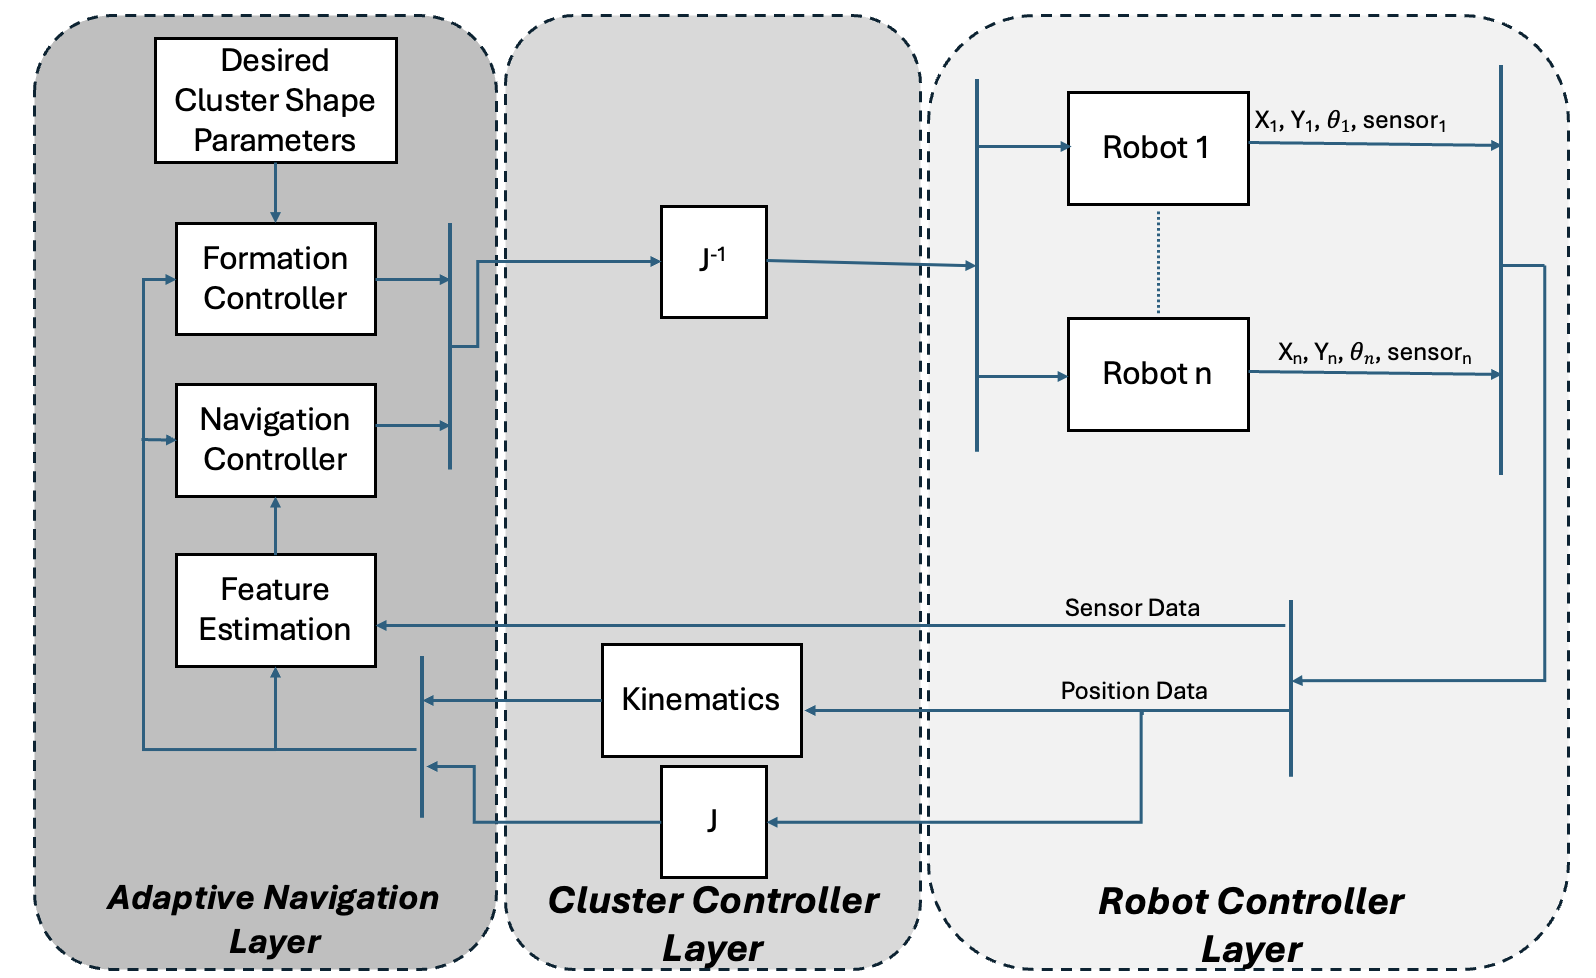
\includegraphics[width=0.40\textwidth]{figures/control_architecture.png}
    \caption{Hierarchical control architecture. Robot controller,
    cluster controller, and adaptive navigation layers, with the state
    control layer sequencing navigation modes above them.}
    \label{fig:control_architecture}
\end{figure}

\subsection{The $D$ Tracker}
\label{sec:sep_controller}

The $D$ tracker drives the cluster centroid onto the trench of $D$ and
then along it, following the separatrix through the crest that separates
one saddle from the next. This is Problem 1. Both motions are built from
the local quadratic surface the estimator returns.

The derivation works in the eigenbasis of the estimated Hessian. Let
$\hat{\mathbf{H}}_{D,0}\mathbf{w}_k = \lambda_k \mathbf{w}_k$ with
$\|\mathbf{w}_k\| = 1$ and $\lambda_1 \leq \lambda_2$. A trench of $D$ is
convex across and concave along, so it is the case
$\lambda_1 < 0 < \lambda_2$. The eigenvector $\mathbf{w}_2$ points across
the trench and $\mathbf{w}_1$ points along it. The sign of an eigenvector
is arbitrary, and the sign of $\mathbf{w}_1$ is fixed so that
$\hat{\mathbf{v}}_0^\top \mathbf{w}_1 \geq 0$, which orients it
downstream.

Because $\hat{D}$ is an exact quadratic surface, the Newton step
$-\hat{\mathbf{H}}_{D,0}^{-1}\hat{\mathbf{g}}_0$ moves in one stroke to
its stationary point. Two properties prevent it from being issued
directly as a velocity command. The first is dimensional, since
$\hat{\mathbf{g}}_0 \approx \hat{\mathbf{H}}_{D,0}\mathbf{r}$ makes the
step a displacement, so commanding it as a velocity asks the cluster to
close the whole remaining distance in one unit of time and diverges as
$\hat{\mathbf{H}}_{D,0}$ approaches singularity. The second is geometric,
in that the stationary point the step seeks is the crest of the trench
rather than a point on the separatrix.

The first is bounded with the hyperbolic saturation
\begin{equation}
    \mathrm{sat}(c) = c_{\max} \tanh\!\left(\frac{c}{c_{\max}}\right),
    \label{eq:sat}
\end{equation}
which trades against a hard clip as follows: it is a bounded transit at
$c_{\max}$ for $|c| \gg c_{\max}$ and transparent for $|c| \ll
c_{\max}$, so one parameter fixes both the transit speed and the width
of the terminal boundary layer, and no per-eigendirection gains are
needed. The second property is addressed by treating the two
eigendirections separately, keeping the Newton component across the
trench and, along it, keeping only its magnitude and taking the
direction from the ambient flow.

That along-trench command changes character at the separatrix. Away from
it the along-trench gradient supplies a descent rate, while on it that
gradient vanishes at the crest even though the separatrix continues
through, so the flow supplies the speed instead. The cluster is declared
on the separatrix,
written $\mathbf{p}_c \in \mathcal{B}$, when
\begin{equation}
    |\hat{D}_0| < \varepsilon_{\mathrm{raw}}
    \quad\text{or}\quad
    \frac{|\hat{D}_0|}{\|\hat{\mathbf{H}}_{D,0}\|_F}
        < \varepsilon_{\dim}.
    \label{eq:flow_band}
\end{equation}
The first test is a raw threshold on the estimated determinant. The
second normalizes it by the local curvature, a ratio with units of length
squared, so the band scales with the landscape rather than with the
absolute size of $D$. The along-trench speed is then
\begin{equation}
    v_\parallel =
    \begin{cases}
        \hat{\mathbf{v}}_0^\top \mathbf{w}_1,
            & \mathbf{p}_c \in \mathcal{B}, \\[6pt]
        \dfrac{|\mathbf{w}_1^\top \hat{\mathbf{g}}_0|}{|\lambda_1|},
            & \text{otherwise},
    \end{cases}
    \label{eq:vpar}
\end{equation}
and the velocity command is
\begin{equation}
    \dot{\mathbf{p}}_c =
    \mathrm{sat}(v_\parallel)\,\mathbf{w}_1
    + \mathrm{sat}\!\left(-\frac{\mathbf{w}_2^\top
      \hat{\mathbf{g}}_0}{\lambda_2}\right)\mathbf{w}_2.
    \label{eq:d_law}
\end{equation}

The two channels are independent. The $\mathbf{w}_2$ term is unaffected
by (\ref{eq:vpar}), so it is the same command on and off the band, and
inside the boundary layer of (\ref{eq:sat}) it is the Newton component of
the fitted quadratic. On the fitted surrogate that step is exact in one
stroke rather than superlinear. Against the true field its rate is set by
how well $\lambda_2$ matches the field's transverse curvature. Since
$v_\parallel \geq 0$ in both branches, the along-trench component of the
motion is never directed against the ambient flow. The $\mathbf{w}_2$
term is unconstrained relative to the flow.

One guard falls outside (\ref{eq:d_law}).
The trench frame is undefined when $\hat{\mathbf{H}}_{D,0}$ has
eigenvalues of one sign, so the law needs a fallback there. Off the
band it reverts to the signed Newton step $\sum_k
\mathrm{sat}(-\mathbf{w}_k^\top\hat{\mathbf{g}}_0/\lambda_k)\mathbf{w}_k$,
which drives the centroid toward the nearest stationary point of
$\hat{D}$ without a stability claim, and on the band it reverts to the
saturated flow alone.

The condition $\lambda_1 < 0 < \lambda_2$ holds of the true field only
where $D$ is concave along the structure, which is a restriction. On the
benchmark, (\ref{eq:gradhess_analytic_main}) gives $D_{yy} = 2\pi^6
A^2\cos 2\pi y_f > 0$ for $|y| > 0.25$, so the true $\mathbf{H}_D$ is
positive definite over the outer half of each separatrix segment and the
trench frame is undefined there. This is geometry rather than accident,
since the flow saddles are local minima of $D$. What supplies the
missing indefiniteness is the estimator. The double gyre satisfies
$u_{xx} = u_{yy}$ and $v_{xx} = v_{yy}$, so $\hat{a}_5 = \hat{a}_6$ and
$\hat{b}_5 = \hat{b}_6$ in the Taylor limit ($\rho \to 0$) and
(\ref{eq:hess_det}) returns $\hat{\mathbf{H}}_{D,0}$ traceless with zero
off-diagonal entry. At finite radius, truncation induces a small trace
(Section~\ref{sec:sensitivity}), so the eigenvalues approximate
$\pm|\hat{H}_{xx}|$ rather than equal it, and the degenerate
case cannot fire. Traversal past a saddle is therefore executed by the
fitted frame outliving the true one rather than by the guard, and a
deliberate relabel-on-saddle rule is the principled version of the same
behavior. It is not implemented here.

\subsection{The $s_1$ Tracker}

This primitive traverses the trench of $s_1$ using four quantities the
fit delivers, the eigenvalue $\hat{s}_1$, its gradient
$\nabla\hat{s}_1$, the strain eigenframe $(\mathbf{e}_1, \mathbf{e}_2)$,
and the deviatoric strain magnitude $r$, which measures how well resolved
that eigenframe is. Remark~\ref{rem:s1hess} rules out a Newton snap on
$s_1$, so both
channels of this primitive are built from the gradient rather than the
curvature.

The first step is to identify the trench tangent. Naming an eigenvector
directly will not work, for the reason given in
Section~\ref{sec:strain_field}. The gradient is used instead. On the
trench, the transverse derivative of $s_1$ vanishes by construction, so
away from a stationary point $\nabla\hat{s}_1$ points almost entirely
along the trench, and the tangent is whichever eigenvector the gradient
is less orthogonal to.
\begin{equation}
    \mathbf{t}_{\mathrm{raw}} =
    \arg\max_{\mathbf{e} \in \{\mathbf{e}_1, \mathbf{e}_2\}}
    \bigl\lvert \nabla\hat{s}_1^\top \mathbf{e} \bigr\rvert,
    \qquad
    \mathbf{t} = \mathrm{sgn}\bigl(\mathbf{t}_{\mathrm{ref}}^\top
    \mathbf{t}_{\mathrm{raw}}\bigr)\,\mathbf{t}_{\mathrm{raw}},
    \label{eq:tangent_select}
\end{equation}
where $\mathbf{t}_{\mathrm{ref}}$ is the previous step's tangent once one
has been established, or the measured flow $\hat{\mathbf{v}}_0$ on the
first tracking step. The rule selects $\mathbf{e}_2$ on the attracting
half of the separatrix and $\mathbf{e}_1$ on the repelling half, swapping
automatically through the origin. Continuity fixes only the residual
sign, not the direction.

The primitive alternates between traversing and settling, selected by a
ride flag $\beta \in \{0,1\}$ that is one while traversing. The velocity
command is
\begin{equation}
    \dot{\mathbf{p}}_c =
    \beta\,c_{\max}\tanh(1)\,\mathbf{t}
    - \mathrm{sat}\!\bigl(g_\perp\,\mathbf{P}\,\nabla\hat{s}_1\bigr),
    \qquad
    \mathbf{P} = \mathbf{I} - \beta\,\mathbf{t}\mathbf{t}^\top,
    \label{eq:oecs_law}
\end{equation}
where $\mathrm{sat}$ acts on a vector by saturating its magnitude and
preserving its direction, reducing to (\ref{eq:sat}) on any scalar
multiple of a unit vector.

This control law decouples descent from travel through the projector.
With $\beta = 1$, $\mathbf{P}$ removes the along-trench component of the
gradient, so the cluster descends only across the trench while riding
along it at cruise speed $c_{\max}\tanh(1)$. With $\beta = 0$, the
projector becomes the identity, the ride term drops out, and the same
expression is full gradient descent on $\hat{s}_1$, which settles at a
local minimum. The gain $g_\perp$ is fixed, standing in for the
curvature normalization that Remark~\ref{rem:s1hess} rules out, so the
transverse channel contracts at gradient rate rather than at Newton
rate.

Two situations clear the ride flag, and they are the state layer's mode
transitions. Before the cluster has reached any structure, $\beta = 0$
and the descent term homes onto the trench from anywhere in the basin.
First contact is declared, and $\beta$ latches to one, when $\hat{s}_1$
first falls below $-s_{\mathrm{trim}}$. The second situation is the
terminal behavior, and it holds the cluster at a two-dimensional
stationary point of $\hat{s}_1$ when
\begin{equation}
    r > r_{\mathrm{band}}, \qquad
    \lVert\nabla\hat{s}_1\rVert < g_{\mathrm{capture}}, \qquad
    \hat{s}_1 < -4 s_{\mathrm{trim}}.
    \label{eq:capture_test}
\end{equation}

A flow saddle is not merely a crossing of two transverse trenches. It is
a genuine two-dimensional minimum of $s_1$, and on the benchmark this
is closed form rather than numerical: (\ref{eq:s1_analytic_main}) gives
$s_1 \geq -\pi^2 A$ with equality exactly at integer $(x_f, y_f)$, a
strict nondegenerate minimum with curvature $\pi^4 A$ on both axes. The
full gradient therefore collapses there, while at an
ordinary trench point the gradient remains large along the trench even
though it vanishes across it. Testing the gradient magnitude is
therefore enough to distinguish the two. This matters because the
ambient flow also stagnates at a saddle, which would starve any
flow-based tangent rule of a direction exactly where the ride needs one.
The three tests in (\ref{eq:capture_test}) reject, in order, the
isotropic point, an ordinary trench point, and a shallow flat spot of
$\hat{s}_1$ away from real structure. The $-4s_{\mathrm{trim}}$ depth
threshold is a hysteresis ratio rather than a physical relation. The
condition arms at four times the first-contact depth and releases when
$\hat{s}_1$ rises back above $-s_{\mathrm{trim}}$, so a noise-driven
flicker of the gradient test does not send the cluster back through the
tangent comparison at the well, while a genuine departure still does.

One guard falls outside (\ref{eq:oecs_law}). If the eigenframe is
degenerate, $r < r_{\mathrm{band}}$, and no previous tangent has been
established, then neither (\ref{eq:tangent_select}) nor continuity
supplies a direction. The command then rides the measured flow,
$\mathbf{t} = \hat{\mathbf{v}}_0/\|\hat{\mathbf{v}}_0\|$, with the
projector set to the identity. Only the first tracking step can reach
this case, and it is the one place in the primitive where the ambient
flow enters the command.

\subsection{Stability Properties}
\label{sec:stability}

The stability properties of the proposed navigation primitives, including
practical stability under bounded estimation error, traversal through
saddle points, and closed-loop frame equivariance, are derived in the
Appendix.

\section{Simulation Program and Results}
\label{sec:results}

\subsection{Simulation Setup}
\label{sec:sim_setup}

A Python simulation implementing the architecture of
Section~\ref{sec:arch} was developed to evaluate both primitives.
The double-gyre experiments use the steady field of
Section~\ref{sec:dg_example} ($A = 0.1$) on the domain $[-1, 1] \times
[-0.5, 0.5]$. The integrator is explicit Euler at 10~Hz ($\Delta t =
0.1$~s), robot dynamics follow the first-order model
(\ref{eq:robot_first_order}), and the cluster layer distributes the
centroid command to the six robots through the analytic $12 \times 12$
inverse Jacobian while driving each of the nine formation shape terms
to its nominal value proportionally (gain 1.0 on lengths, 0.1 on
angles, fixed across all experiments). All trials use the nominal
formation with ring radius $\rho = 0.075$; a trial varies only the
formation's initial heading, drawn uniformly from $[0, 2\pi)$ in the
Monte Carlo sweeps and zero in the noise-free demonstration runs. The
cluster's angular velocity command is zero throughout every run, so
heading is held fixed at its draw, and the reported
ring-phase-dependent quantities are with respect to it. Clean trials
run 400 to 600 steps and stop at domain exit or, for the $D$ tracker,
150 steps after first saddle contact. Noise-sweep trials run up to 500
steps and stop at task completion or domain exit. The
estimator-accuracy sweep holds the formation static and draws
independent noise per trial.

Four experiment families exercise the primitives: noise-free
double-gyre runs from six matched starts, Monte Carlo sweeps over a
two-dimensional noise grid, a rotating-observer trial, and runs on a
measured ocean record. Each is described with its results below.

\subsection{Ocean HFR Setup}
\label{sec:ocean_sim}

The ocean experiment uses hourly surface-current frames for the Santa
Barbara Channel from the HFRNet U.S.~West~Coast Radial-to-Total Vector
product \cite{40}, on the $2$~km grid. The record is the same one
\cite{17} uses for its own Santa Barbara Channel experiment, the same
network over the same 28-h window, 29 frames from May 16, 2012 08:00
GMT to May 17, 2012 12:00 GMT, so these results are interpretable
against prior work on this record; no controlled head-to-head against
\cite{17} was run, since initialization and advection differ. Frames
are interpolated linearly in time inside the field evaluator. World
coordinates on $[-0.65, 0.65]^2$ map affinely onto a region centered on
$(34.2^{\circ}\mathrm{N}, -120.4^{\circ}\mathrm{W})$ spanning
$\pm 0.300^{\circ}$ of latitude and $\pm 0.363^{\circ}$ of longitude. The
$168$-step trial spans the full record.

Every physical number reported for this field comes from one unit block.
The length unit is $L_w = 51.4$~km on both axes. The time unit is
$6000$~s. The control period is $\Delta t = 0.1$ time units, so one
simulated step advances the field by $600$~s and the $168$-step trial
covers the $28$-h record. The two together fix the derived units: one
world unit of velocity is $L_w/6000\,\mathrm{s} = 8.56$~m/s, and one
world unit of strain rate, vorticity, or any other Jacobian entry is
$1/6000\,\mathrm{s} = 1.67 \times 10^{-4}$~s$^{-1}$. The saturation
$c_{\max} = 0.04$ is therefore $0.34$~m/s and the commanded-speed cap
$\sqrt{2}\,k\,c_{\max}$ is $0.87$~m/s. Because
$\alpha_{\text{mom}} = 0$ here, the discrete bound of
Appendix~\ref{app:stability} is
the tighter $\Delta t\,k\,a_\perp < 2$, which at $\Delta t = 0.1$ and
$k = 1.8$ admits transverse rates up to $a_\perp = 11.1$ in these
units. The FTLE fields used for evaluation are computed from subwindows
of this same record, at two horizons. The 24-h field of
Fig.~\ref{fig:ocean_ftle} integrates the first 25 frames, 08:00 GMT
May 16 to 08:00 GMT May 17. The four-anchor persistence check
uses a 12-h horizon.

The longitude half-extent is $0.3^{\circ}/\cos(34.2^{\circ})$, so both
axes carry the same physical scale and the map is a similarity, a
uniform dilation of the local tangent plane. With
$\mathbf{J}_{\mathrm{world}} = L_w \mathbf{J}_{\mathrm{phys}}$ the
determinant scales by $L_w^2$ and the symmetric part by $L_w$, both
positive constants, so sampled vector directions, every zero set,
trench, and extremum of $D$, and the rate-of-strain eigenframe are the
physical ones. The tangent plane uses the same constants as the FTLE
reference, so the controller frame and the evaluation frame agree by
construction.

The ocean operating point follows, and each departure from the
double-gyre column is a trade against a named quantity. The pentagon is
enlarged to $\rho = 0.105$, $1.4\times$ the nominal radius and $5.4$~km
at this site, trading truncation bias for noise suppression so that the
six-robot footprint spans about five cells of the $2$~km grid rather
than under four. At one control cycle per ten minutes any vessel time
constant is negligible, so $\alpha_{\text{mom}} = 0$, and the stiction
floor drops to $0.002$, a motor-friction floor with no vessel-scale
analogue. The navigation gain $k = 1.8$ follows the ridge branch that
makes landfall on the middle island. No noise level is estimated
for this field. The exactly-determined six-robot fit leaves no residual
to estimate $\sigma_{uv}$ from, and quantifying the uncertainty in
actual ocean data and its impact on the proposed tracking strategy is,
as \cite{17} concludes for this same record, a substantially harder
problem left outside its scope. The noise model used in this paper is
validated on the double gyre only.

\subsection{Estimator Accuracy}
\label{sec:results_est}

\begin{figure}[!t]
    \centering
    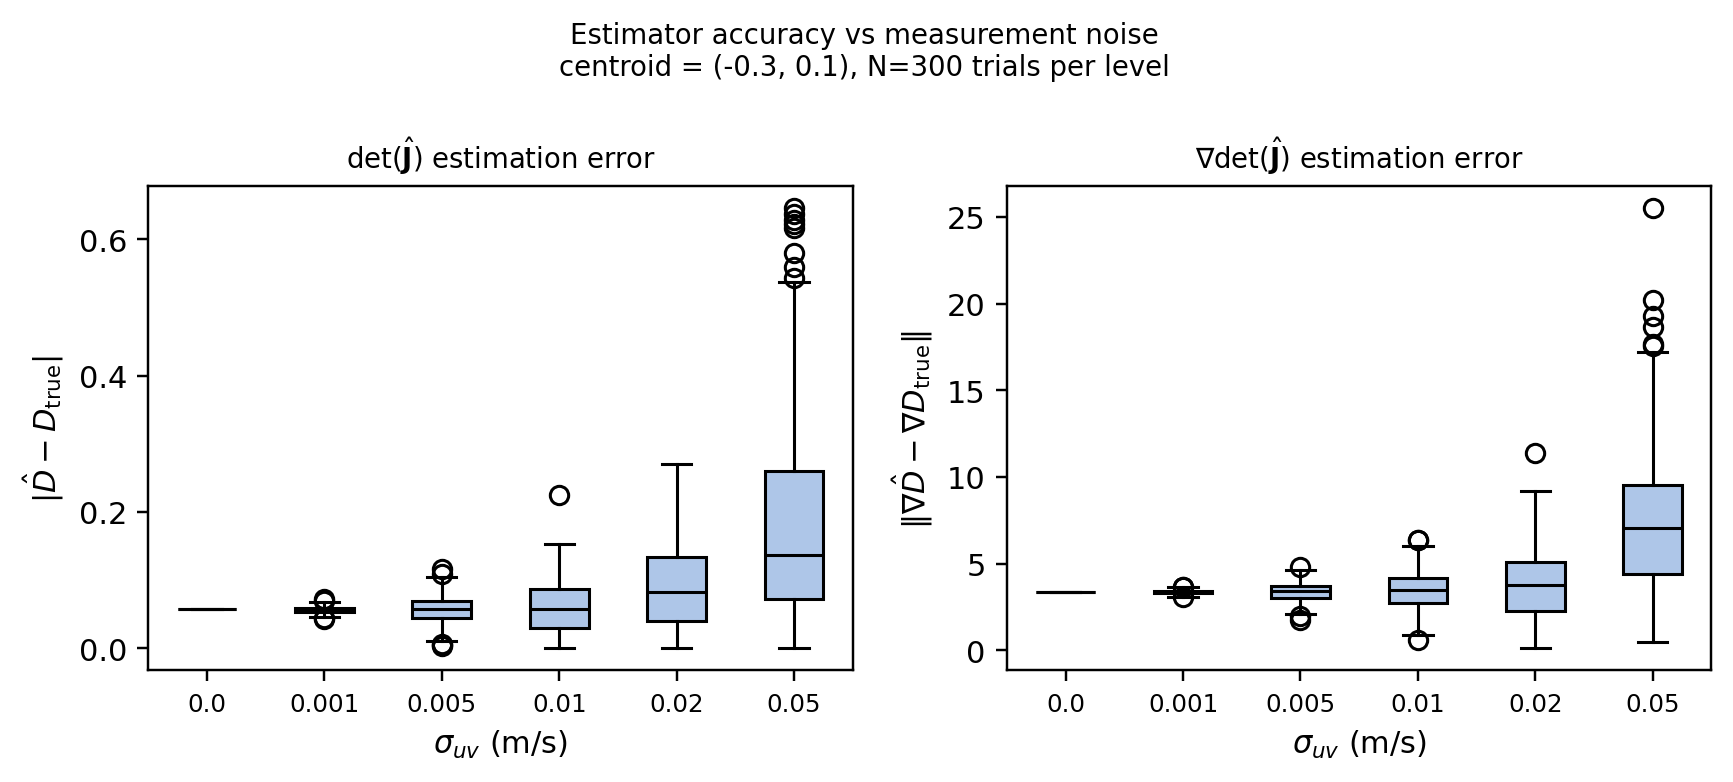
\includegraphics[width=0.9\columnwidth]{figures/estimator_accuracy_vs_noise.png}
    \caption{Estimator accuracy on the steady double gyre at the strain-region
    point $(-0.3, 0.1)$, $10^4$ noise draws per point. (a) Median relative error
    of $\hat{D}$, $\nabla\hat{D}$, and $\hat{\mathbf{H}}_D$ against measurement
    noise at $\rho = 0.075$. The dashed line marks error equal to signal, the
    dash-dotted line the noise at which closed-loop traverse success crosses
    50\% (Table~\ref{tab:mc_success}(a)). (b) Mean angle between the fitted and
    the true principal eigenvector of $\hat{\mathbf{H}}_D$, against the
    $45^\circ$ expected of a uniformly random axis. The star is truncation
    acting alone.}
    \label{fig:est_accuracy}
\end{figure}

The estimator was characterized on the steady double gyre before any loop
was closed, over $10^4$ draws per condition at the strain-region point
$(-0.3, 0.1)$. Every prediction of Section~\ref{sec:sensitivity} held.
Coefficient standard deviations matched (\ref{eq:gain_ladder}) within
2.1\%, the reading error induced by position noise matched
(\ref{eq:sigma_eff}) within 1.6\%, the downward bias of $\hat{s}_1$ matched
(\ref{eq:s1_bias}) within 5\% in eighteen of twenty-four conditions and
within one standard error of the sample mean in all twenty-four, the six
wider cases being those at $r/\sigma_r \geq 3$ where the predicted bias
is itself below the resolution of $10^4$ draws, and
the signed mean error of $\hat{D}$, $\nabla\hat{D}$, and
$\hat{\mathbf{H}}_D$ was zero to within 2.7\% of one standard deviation
across forty-eight conditions, as Proposition~\ref{prop:unbiased} requires.
The correlation between the two component errors at one robot was $0.41$
under position noise against $0.44$ predicted, and zero under measurement
noise, which is the mechanism separating the channels.

In Fig.~\ref{fig:est_accuracy}(a), $\hat{D}$ stays informative to
$\sigma_{uv} \approx 0.07$ and $\nabla\hat{D}$ to $\approx 0.0075$, while
$\hat{\mathbf{H}}_D$ never falls below the error-equals-signal line at any
noise level, held there by $e_H$. In Fig.~\ref{fig:est_accuracy}(b),
truncation acting alone costs the $\hat{\mathbf{H}}_D$ eigendirections
$2.2^\circ$, while noise costs them $24^\circ$ by $\sigma_{uv} = 0.003$ and
$39^\circ$ at the closed-loop failure cliff, against $45^\circ$ for a
uniformly random axis.

The $s_1$ channel was checked at the nominal radius against its analytic
values, drawing $10^4$ realizations per condition at a fixed
strain-region point. The fitted shear strain at three test points is at
the $10^{-4}$ level (analytic value zero), and the fitted
$\hat{\mathbf{H}}_{s_1}$ eigenvalues are $[-0.011, 0.000]$ and smaller,
negative semidefinite as Remark~\ref{rem:s1hess} requires. The
transverse component of (\ref{eq:grad_s1}) at $(0.03, 0.25)$, averaged
over ring phase, recovers a restoring slope of $6.83$ against the
analytic transverse curvature $6.888$, a full-sweep mean of $0.9$\%
truncation deficit. The spread across phases is the orientation
dependence of Section~\ref{sec:sensitivity} rather than scatter.
Rotating the ring through its $72^\circ$ period at the same point moves
the recovered slope between $4.0$ and $9.7$ about that mean of $6.83$,
and halving $\rho$ halves the spread, confirming the linear-in-radius
scaling. The mean tracks the analytic value, so the estimator is not
biased in the transverse channel. An individual formation orientation
is. At $\sigma_{uv} = 0.01$ the median direction error of
$\mathbf{e}_2$ is $4.5^\circ$, against $44^\circ$ for $\nabla\hat{s}_1$
and $41^\circ$ for the $\hat{\mathbf{H}}_D$ eigenvector ($2\times 10^4$
draws per level).

\subsection{Clean Runs}
\label{sec:disc_clean}

\begin{figure}[!t]
    \centering
    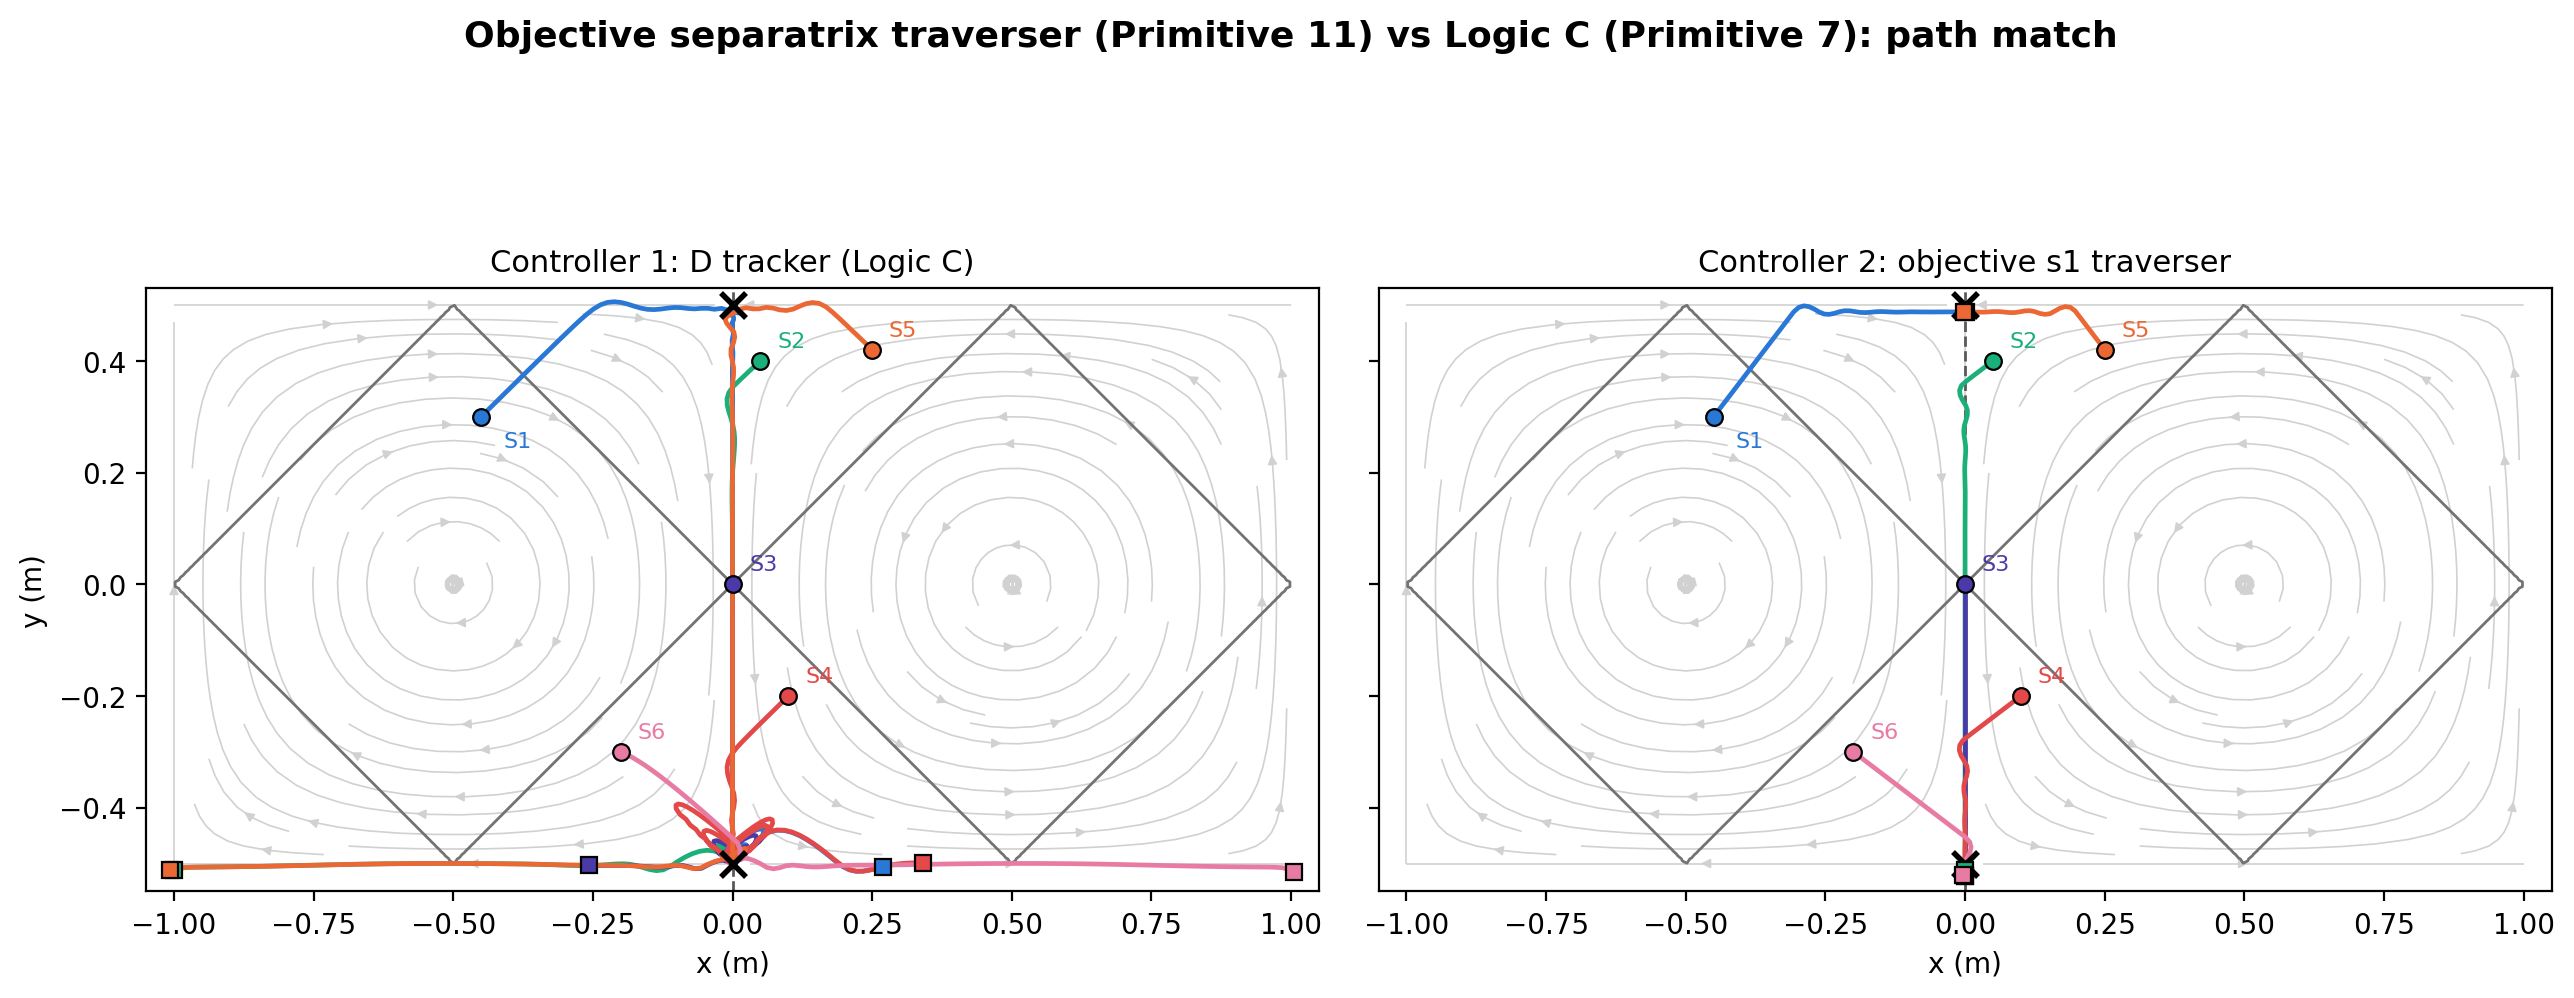
\includegraphics[width=0.44\textwidth]{figures/traverse_vs_logic_c.png}
    \caption{$s_1$ tracker versus $D$ tracker from six matched starts
    ($\bullet$), noise-free, overlaid on the double-gyre streamlines and
    Okubo-Weiss diamonds. Both traverse the same network through the
    isotropic point at the origin. The $s_1$ tracker captures at the
    saddle ($\times$) its tangent orientation resolves toward, while the
    $D$ tracker continues onto the crossing wall trench past every saddle
    it reaches, ending at the square markers.}
    \label{fig:traverse_vs_logic_c}
\end{figure}

Both primitives were run noise-free from the same six starts
(Fig.~\ref{fig:traverse_vs_logic_c}), spanning both gyre halves, the
origin, and points off the structure entirely, between $0$ and $2.7\rho$
from the nearest trench segment ($\rho = 0.075$, the formation radius).
Each run records the step at which the centroid first reaches the trench
and holds it, the closest approach to each saddle, and whether the run
settles at a saddle or continues through it onto the crossing wall
trench. Both acquire the trench network from every start, in 6 to 35
steps for the $D$ tracker and 0 to 46 for the $s_1$ tracker, then ride
the same segments in the same direction and cross the isotropic point at
the origin. A run acquiring above the origin therefore rides an
attracting OECS to that point and continues onto a repelling one, on the
same law and the same scalar trench throughout.
Theorem~\ref{thm:separatrix} does not distinguish them: the normal form
is written for either surrogate and both laws command the same
transverse dynamics. Where the two commit to the same saddle the paths
are visually coincident, and the mean path gaps of 0.020 to 0.322 over
the common on-trench portion open only where they commit to different
ones. Neither needs dedicated machinery at the crossing. The $s_1$
tracker rides through the origin on ordinary tangent selection
(\ref{eq:tangent_select}), and over a sweep of $r_{\text{band}}$ from
0.05 to 0 the degenerate-frame guard never fires once.

By the fourth consequence of the splitting identity
(\ref{eq:trench_coincide}, Section~\ref{sec:detj_field}), the two trenches
coincide wherever the vorticity vanishes and the flow is
strain-dominated. The double gyre's entire
trench network is such a set, the vorticity of
Section~\ref{sec:dg_example} being identically zero on the separatrix
$x_f = 1$ and on all four walls. The lone exception is the isotropic point
at the origin, where $\mathbf{J}$ vanishes entirely and the step from
(\ref{eq:trench_coincide}) is unavailable. The six clean runs therefore
agree pointwise for a reason specific to this field, not because the two
surrogates are interchangeable in general.

The primitives part only at the terminal step, and the split is a fact
about the model class rather than about tuning. The $s_1$ tracker
settles within 0.011 to 0.022 of a saddle in every run, at whichever one
its initial tangent orientation resolves toward, four at
$\mathbf{p}^*_1 = (0, -0.5)$ and two at $\mathbf{p}^*_2 = (0, 0.5)$. The
$D$ tracker passes within 0.02 of $\mathbf{p}^*_1$, then rides onto the
crossing wall trench and continues, because the capture test
$\lambda_1\lambda_2 \geq 0$ cannot fire. This
is not a noise floor and not a tuning margin. By
Section~\ref{sec:sep_controller} the fitted $\hat{\mathbf{H}}_D$ is
traceless on this field, so its eigenvalues approximate
$\pm|\hat{H}_{xx}|$ on the network, the induced trace being a
finite-radius truncation artifact that varies with ring phase. At the
well, at the mirror-antisymmetric ring phase, the estimated pair is
$[-0.51, 0.45]$ against a true $[18.3, 19.2]$; at the worst phase
$18^\circ$ away it is $[-0.72, 0.43]$, which is the floor $e_H$
at $|y| = 0.45$. The same
limit binds in both directions, since $\hat{\mathbf{H}}_{s_1}$ is
negative semidefinite for every field and formation
(Remark~\ref{rem:s1hess}), so neither surrogate admits a definiteness
certificate. The one terminal test a quadratic fit supports is a
vanishing gradient, and a flow saddle is a genuine two-dimensional
minimum of $s_1$, so that test is sufficient exactly where the $s_1$
tracker needs one and unavailable where the $D$ tracker would need one.
Traversal and capture are the same representability limit read twice.

The clean-field descent also fixes the reachable set, and it is not the
Okubo-Weiss partition. Over a 20\,000-cell start-position grid,
distinct from the separate 20\,000-trial acquisition sweep reported in
Section~\ref{sec:disc_noise}, no
run settles at a gyre core, so descent of $\hat{D}$ leaves the
rotation-dominated interiors rather than stalling in them. The
reachable set is the watershed of that descent composited with the flow
direction on the acquired branch, whose arrival rate at
$\mathbf{p}^*_1$ is 47.4\% over that grid and 47.1\% over $n =
10{,}000$ uniformly random starts and headings. Prior AN primitives
\cite{3}, \cite{4} report local convergence without such an estimate.

A spot check on the time-varying double gyre
(\ref{eq:dg_unsteady}) \cite{17}, at
$\varepsilon = 0.1$ and $\omega_{dg} = 2\pi/10$ against the static
$\varepsilon = 0$ used everywhere else, runs the $D$ tracker down the
oscillating trench at zero noise. The trench swings $\pm 0.116$ in $x$
with peak speed equal to 62\% of the commanded speed cap, and the
primitive holds it with mean transverse offset 0.006 and maximum 0.015,
with no time-derivative term in the controller and no analytic
guarantee for that case.

\subsection{Behavior Under Noise}
\label{sec:disc_noise}

\begin{table}[!t]
\centering
\caption{Monte Carlo traverse success (\%), 10\,000 trials per cell
from the straddling start $(0, 0.35)$ with a random heading per trial,
for the (a) $D$ and (b) $s_1$ trackers. Both are scored against the
single far saddle $\mathbf{p}^*_1$ a noise-free run from this start
reaches. At 10\,000 trials/cell the 95\% confidence half-width on any
reported percentage is under 1 point.}
\label{tab:mc_success}
\footnotesize
\setlength{\tabcolsep}{4.5pt}
\begin{tabular}{@{}l|rrrrr@{}}
\hline
& \multicolumn{5}{c}{$\sigma_p$} \\
\cline{2-6}
$\sigma_{uv}$ & 0.000 & 0.005 & 0.010 & 0.020 & 0.050 \\
\hline
\multicolumn{6}{@{}l}{(a) $D$ tracker} \\
0.000 & 100.0 &  65.7 &  44.5 &  33.3 &  19.0 \\
0.001 &  99.6 &  63.2 &  45.6 &  32.9 &  19.1 \\
0.005 &  62.4 &  52.1 &  43.5 &  31.2 &  19.4 \\
0.010 &  43.7 &  40.7 &  37.0 &  28.8 &  18.7 \\
0.020 &  25.5 &  25.7 &  24.3 &  22.6 &  17.0 \\
0.050 &  16.0 &  16.2 &  15.8 &  16.1 &  14.9 \\
0.100 &  14.1 &  14.1 &  14.3 &  14.6 &  13.6 \\
0.200 &  13.5 &  12.4 &  12.8 &  12.8 &  12.4 \\
0.400 &  12.1 &  12.2 &  12.0 &  12.3 &  11.9 \\
0.800 &   4.8 &   5.4 &   5.1 &   5.4 &   5.2 \\
\hline
\multicolumn{6}{@{}l}{(b) $s_1$ tracker} \\
0.000 & 100.0 &   1.3 &   0.0 &   0.0 &   0.0 \\
0.001 &  91.8 &   1.1 &   0.0 &   0.0 &   0.1 \\
0.005 &   0.0 &   0.0 &   0.0 &   0.0 &   0.0 \\
0.010 &   0.0 &   0.0 &   0.0 &   0.0 &   0.0 \\
0.020 &   0.0 &   0.0 &   0.0 &   0.0 &   0.1 \\
0.050 &   0.2 &   0.2 &   0.1 &   0.1 &   0.1 \\
0.100 &   0.5 &   0.4 &   0.4 &   0.4 &   0.3 \\
0.200 &   0.5 &   0.4 &   0.6 &   0.4 &   0.4 \\
0.400 &   0.5 &   0.5 &   0.5 &   0.6 &   0.5 \\
0.800 &   0.5 &   0.7 &   0.4 &   0.6 &   0.5 \\
\hline
\end{tabular}
\end{table}

\begin{figure}[!t]
    \centering
    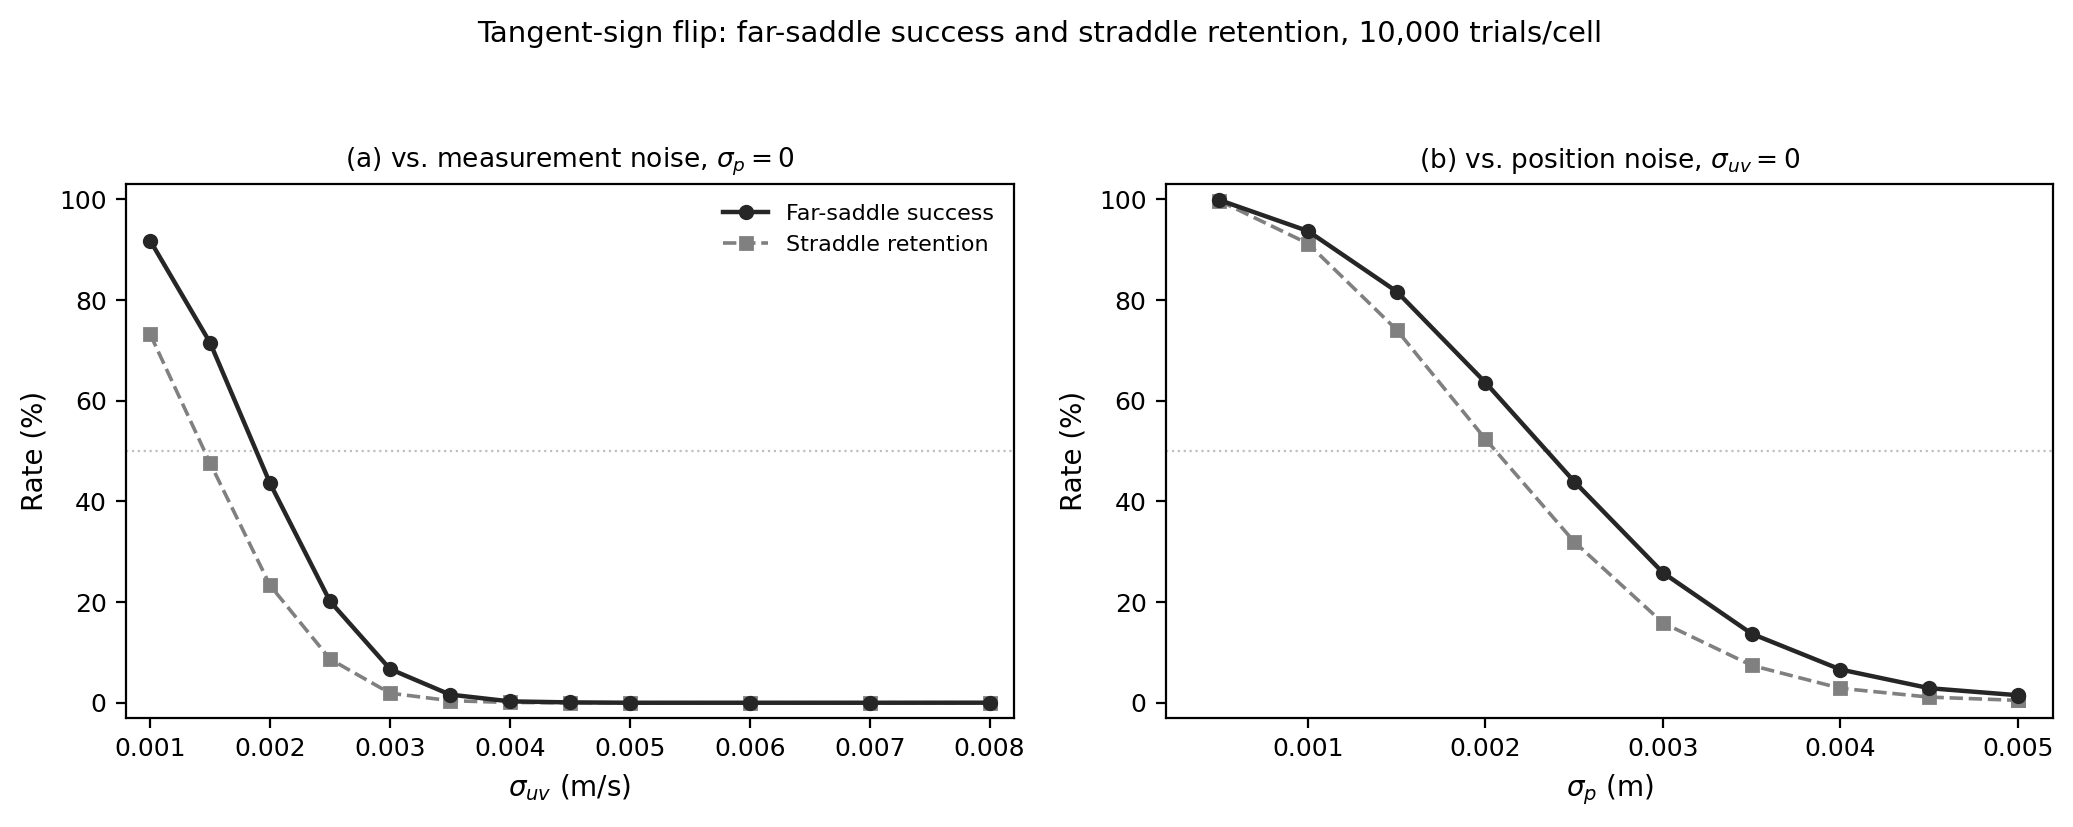
\includegraphics[width=0.9\columnwidth]{figures/flip_resolution.png}
    \caption{Resolving the tangent-sign flip. Far-saddle success and
    straddle retention (both conditioned on reaching $\mathbf{p}^*_1$),
    10\,000 trials/cell, at 0.0005 spacing on each axis. (a) Against
    $\sigma_{uv}$, $\sigma_p = 0$. Success crosses 50\% between
    $\sigma_{uv} = 0.0015$ and 0.002 and reaches a sub-1\% floor by
    0.005, held out to 0.008. (b) Against $\sigma_p$, $\sigma_{uv} = 0$.
    The same decline, crossing 50\% between $\sigma_p = 0.002$ and
    0.0025. The transition is resolved and continuous on both axes; what
    is abrupt is the outcome it selects between, since runs on either
    side of it settle at a saddle with comparable reliability and differ
    in which one.}
    \label{fig:flip_resolution}
\end{figure}

Both primitives sweep the same two-dimensional noise grid from one
straddling start, $(0, 0.35)$, so the success rate measures noise
robustness rather than basin geometry. The grid spans $\sigma_{uv} \in
\{0,\, 0.001,\, 0.005,\, 0.01,\, 0.02,\, 0.05,\, 0.1\}$, with the top
level doubled and re-swept while the worst cell still succeeds above
10\% ($\sigma_{uv} = 0.8$), and $\sigma_p \in \{0,\, 0.005,\, 0.01,\,
0.02,\, 0.05\}$, at 10\,000 trials per cell of at most 500 steps, each
from an independent initial heading. Success is contact within 0.06 of
the far saddle $\mathbf{p}^*_1 = (0, -0.5)$, which a noise-free run
from this start reaches under either law, without formation collapse
(root-mean-square error of the fifteen inter-robot distances from
nominal above 0.30, four times $\rho$). Holding one target fixed for
both surrogates makes a settle at the near saddle a directional failure
rather than a loss of the structure. Each trial also records straddle
retention (robots on both sides of the separatrix from first straddle
to stop, the failure count of \cite{17}) and tracking error (mean of
$|x_c|$).

Table~\ref{tab:mc_success} reports traverse success for both primitives
over that grid, scored against $\mathbf{p}^*_1$. Noise separates the two
and it favors the $D$ tracker, whose 50\% crossing sits a full grid step
later, and the two do not fail the same way.

For the $D$ tracker the cliff and an estimator threshold nearly coincide.
Success holds at 100\% with no noise and crosses 50\% at $\sigma_{uv}
\approx 0.0079$, within 5\% of the $\sigma_{uv} \approx 0.0075$ at which
$\nabla\hat{D}$ stops being informative (Section~\ref{sec:results_est}).
The gradient is not the only input that has run out by then.
Fig.~\ref{fig:est_accuracy}(b) puts the curvature eigenframe $39^\circ$
from truth at the cliff, against $45^\circ$ for a uniformly random axis,
and past $24^\circ$ by $\sigma_{uv} = 0.003$. Both terms of
(\ref{eq:d_law}) are built on that frame and normalized by its
eigenvalues, so the command inherits the degradation in full. This is
separate from the floor $e_H$ of Section~\ref{sec:sensitivity}, which on
the benchmark is available in closed form. Substituting (\ref{eq:dg_u})
into (\ref{eq:hess_det}) gives, on the separatrix,
\begin{equation}
    \hat{H}_{xx} = 2\pi^6 A^2 \sin^2 \pi y_f,
    \qquad
    e_H = 2\pi^6 A^2 \cos^2 \pi y_f,
    \label{eq:floor_closed}
\end{equation}
against the true $D_{xx} = 2\pi^6 A^2$ of
(\ref{eq:gradhess_analytic_main}). The fit recovers the transverse
curvature at the crest and loses almost all of it at the saddles, $e_H$
reaching $98$\% of $D_{xx}$ at $|y| = 0.45$. The floor falls on the
eigenvalues and leaves the eigendirections nearly intact, so it is not
what degrades the frame. The directions are resolved instead by
the eigenvalue separation against the entry noise
(\ref{eq:gain_ladder}) places at $\nu/\tilde{\rho}^{\,2}$, and once that
noise reaches the separation the recovered frame is uniform. Neither
threshold is a property of (\ref{eq:d_law}), so the estimator sets the
noise ceiling.

Three readings sit alongside it. Position noise scales the
estimator-accuracy curve by $\|\mathbf{J}\|$ per (\ref{eq:sigma_eff}), so
$\sigma_p = 0.01$ alone and $\sigma_{uv} = 0.01$ alone give nearly
identical rates. Beyond the cliff success levels off in the low tens of
percent through $\sigma_{uv} = 0.2$ rather than falling to zero, an
unbiased-random-walk floor that decays only at $\sigma_{uv} = 0.8$, while
straddle retention, the failure metric of \cite{17}, decays cleanly with no
such floor (1.000, 0.589, and 0.389 at $\sigma_{uv} = 0$, 0.005, and 0.01).
Acquisition is not the noise-limited phase either, the cluster reaching
the trench network within 0.05 in every one of 20\,000 acquisition
trials through $\sigma_{uv} = 0.02$, swept from two clean-run starts
$2.7\rho$ off the structure.

The $s_1$ tracker fails earlier, for a reason that has nothing to do with
estimator accuracy. Its success
falls from 91.8\% at $\sigma_{uv} = 0.001$ through
43.5\% at 0.002 to 0.0\% by 0.005, a floor it holds out to 0.008, where the
$D$ tracker's corresponding column, over the wider interval
$\sigma_{uv} \in [0.005, 0.010]$, falls only from 62.4\% to 43.7\%. The
$s_1$ tracker's floor sits at zero rather than in the low tens of
percent because capture settles wherever the ride stops rather than
continuing past it: once the tangent sign has laundered to the wrong
branch there is no further wandering to random-walk back, so the
failure is total rather than partial.
Fig.~\ref{fig:flip_resolution} resolves the transition at 0.0005
spacing on each noise axis separately, and the two panels are one finding
measured twice rather than two failure modes, since position noise enters
the same comparison through the coupling
$\mathbf{J}(\mathbf{p}_i)\boldsymbol{\xi}_i$ of (\ref{eq:pos_noise}) and
$\|\mathbf{J}\| \approx 1$ at this test point. The cluster has not lost
the structure, become erratic, or collapsed. It rides the separatrix
competently and settles, in the wrong direction. This is a sign
inversion rather than a decay toward chance, which is what makes the
far-saddle column the score that separates the two outcomes, since a
near-saddle settle is indistinguishable from a success in every other
recorded quantity.

The mechanism is the eigenvector comparison in
(\ref{eq:tangent_select}), not the flow read that seeds
$\mathbf{t}_{\text{ref}}$. The seed is the better conditioned of the two,
since the fit interpolates at the center robot and $\hat{\mathbf{v}}_0$
therefore carries noise $\sigma_{uv}$ with $\gamma_0 = 1$, giving a
signal-to-noise ratio of $71$ at $\sigma_{uv} = 0.002$ against the flow
of $0.1426$ at this start. The continuity rule cannot reverse a tangent
in one step either (Theorem~\ref{thm:separatrix}), and instrumented runs
count no one-step reversal at any
level swept. The argmax is where the margin actually is. On the
separatrix $s_s \equiv 0$ and $\mu \equiv 0$, so (\ref{eq:grad_s1})
collapses to $\nabla\hat{s}_1 = \pm(\hat{a}_5, \hat{a}_4)$ with the
eigenvectors on the coordinate axes, reducing
(\ref{eq:tangent_select}) to the comparison $|\hat{a}_5| > |\hat{a}_4|$.
The true $a_5 = u_{xx}$ is identically zero there and $a_4 = -\pi^3 A
\sin \pi y_f$ collapses at both saddles, so the test weighs a quantity
whose true value is zero against one that vanishes where the ride ends,
deciding with the largest noise gain in (\ref{eq:gain_ladder}). Its
signal-to-noise ratio here, against the combined noise of the two
compared coefficients, is $1.4$ at $\sigma_{uv} = 0.002$ (against
$\sigma(\hat{a}_4)$ alone it is $3.13$), fifty times
worse than the seed's.

Supplying one channel at a time from noise-free values separates them.
Giving the seed its clean flow moves the correct-saddle rate at
$\sigma_{uv} = 0.002$ from 44.6\% to 45.8\% (10\,000 trials/cell). Giving
the argmax its clean gradient and eigenframe moves it to 100\% at both
$\sigma_{uv} = 0.002$ and $\sigma_{uv} = 0.005$, where the unaided
primitive is at zero. The sign is therefore
laundered rather than flipped. The argmax hops to the transverse
eigenvector, continuity resolves that hop against a direction orthogonal
to the trench, which carries no information about which way the trench
runs, and the hop back inherits a sign that is now a coin flip. Hop rates
run at 2.4\% of tracking steps at $\sigma_{uv} = 0.001$ and 13.3\% at
0.002, tracking the inversion rate, and moving the start to $(0, 0.15)$,
where $|\nabla s_1|$ is larger and the competitor still identically zero,
shifts the 50\% crossing from between 0.0015 and 0.002 to between 0.003
and 0.0035 with nothing else changed. The exposure therefore sits at the
saddles, where $\nabla s_1$ collapses, and not at the isotropic point,
where it is largest. That is the same quantity
(\ref{eq:capture_test}) relies on for capture, so the capture test
becomes reliable exactly where the tangent rule stops being, and the
clean-run finding that the guard never fires at the origin
(Section~\ref{sec:disc_clean}) says nothing about the noisy case.

The zero-noise tracking errors, 0.0075 for the $s_1$ tracker against
0.0016 for the $D$ tracker, have a separate cause. Both primitives park
where their own transverse command vanishes, which is where the
\emph{fitted} trench lies rather than the field's, and the gap between
the two is the orientation-dependent truncation bias of
Section~\ref{sec:sensitivity}. Solving for that offset from the
open-loop fit alone, with no closed loop and no gains, predicts
trial-mean $|x_c|$ of 0.0079 and 0.0019 against those measurements,
averaged over ring phase. Success is not anisotropic in the same way,
staying within 75.9--77.1\% across initial-heading quartiles over the
40\,000 trials at $\sigma_{uv} \leq 0.01$, because the bias displaces
the ride without threatening it. Neither primitive shows the signature
of the discrete bound: trajectories at the worst orientation hold a
smooth one-sided offset over the portion of a 300-step run where
$\Delta t\,k\,a_\perp$ exceeds 12, where a limit cycle would change
sign every step or two. Two independent reasons account for the
absence, and both should be given. The cluster is only briefly in that
regime, since $\Delta t\,k\,a_{\perp,D} > 12$ requires $|y| > 0.4495$,
the last 5\% of a separatrix segment; and while it is there the
proportional band $c_{\max}/a_\perp = 0.0011$ is smaller than the
measured tracking error 0.0016, so the linearization the
actuator-aware threshold of Appendix~\ref{app:stability} comes from
never applies.

The general reading is about where a decision is anchored rather than how
accurately it is read. The direction the $s_1$ tracker rides is the
better estimated of the two tangent sources by an order of magnitude in
angle (Section~\ref{sec:results_est}), and it is still the less robust
primitive here. The $D$
tracker re-signs $\mathbf{w}_1$ against $\hat{\mathbf{v}}_0$ on every
cycle, so a corrupted frame costs it one cycle, but that reference is not
free of the exposure Section~\ref{sec:sep_controller} raised against a
flow-based rule: $\hat{\mathbf{v}}_0$ collapses at the same saddle
stagnation point the $s_1$ tracker's gradient test was built to avoid
consulting. The clean runs already bound the consequence, since a single
miscue is overwritten the very next cycle instead of being carried
forward. The $s_1$ tracker
consults the flow once and thereafter carries the sign in state through
$\mathbf{t}_{\text{ref}}$, so the sign survives no longer than the chain
of comparisons that propagates it, and one hop through an orthogonal
intermediate breaks the chain without any single comparison being
reversed. Robustness is set
less by the per-cycle accuracy of what a
law reads than by how far a decision is carried before it is checked
against the world again.

\subsection{Behavior Under a Rotating Observer}
\label{sec:objectivity_tradeoff}

\begin{figure}[!t]
    \centering
    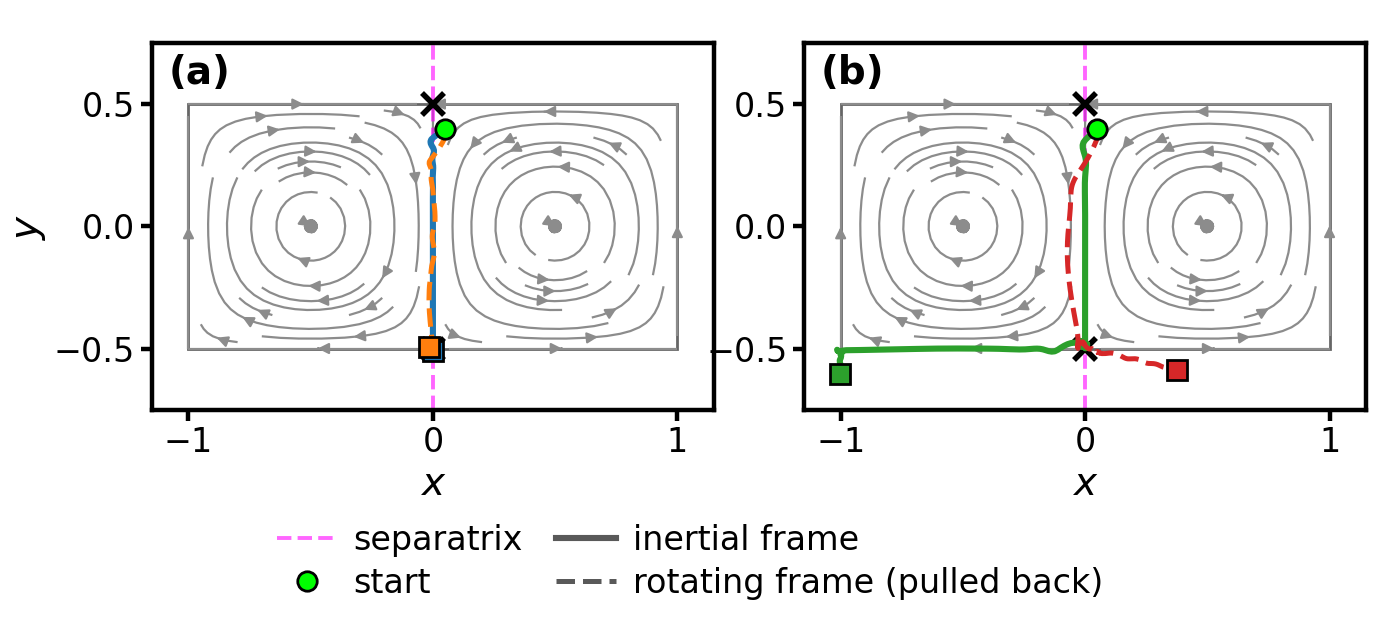
\includegraphics[width=\columnwidth]{figures/objectivity_traverser.png}
    \caption{Objectivity trial, both primitives started from
    $(0.05, 0.40)$. Each is run in the inertial frame (solid) and in a
    frame rotating at $\Omega = 0.2$ rad/s (dashed, pulled back to
    inertial coordinates). (a) the $s_1$ tracker's two runs coincide
    along the whole separatrix and capture at the same saddle (final gap
    0.025). (b) the $D$ tracker's rotating-frame run leaves the
    separatrix (final gap 1.219), the artifact predicted by
    (\ref{eq:D_not_objective}).}
    \label{fig:oecs_objectivity}
\end{figure}

Both primitives were run from $(0.05, 0.40)$, just inside the upper
saddle, on the same physical double gyre expressed in two observer
frames, the inertial frame and a frame rotating at $\Omega = 0.2$
rad/s, in which the field is $\mathbf{v}'(\mathbf{p}', t) =
\mathbf{Q}\mathbf{v}(\mathbf{Q}^\top \mathbf{p}') + \Omega\,(-y',
x')^\top$. The strength of the rotation relative to the field is set by
the Rossby number, the field's own vorticity scale against the frame's,
$\mathrm{Ro} = \lvert\omega\rvert_{\max}/2\Omega$, so that small
$\mathrm{Ro}$ is rotation dominated. The double gyre's peak vorticity is
$2\pi^2 A \approx 1.97$ against an added solid-body vorticity $2\Omega =
0.4$, giving $\mathrm{Ro} \approx 4.9$. The frame is therefore a
perturbation on the vorticity scale and not on the scale of $D$, where
its effect is unbounded. The rate keeps the structure's apparent speed
at the tracked radius, $\Omega r \leq 0.10$, inside the command
authority $k\,c_{\max} = 0.12$, the condition
Proposition~\ref{prop:equivariance} requires of the closed loop.
Rotating-frame trajectories are pulled back to inertial coordinates and
compared with the inertial run of the same primitive.

The trial reverses the ranking, and not by a margin
(Fig.~\ref{fig:oecs_objectivity}). The $s_1$
tracker's two runs are the same material path, final gap 0.025 and mean gap
0.014, with mean distance to the true trench network of $1.5\times 10^{-7}$
inertial against 0.0048 rotating, both capturing at the same bottom saddle.
This distance is measured to the nearest trench line along a single
deterministic run at zero initial heading, not the $|x_c|$ transverse
offset the noise sweeps of Section~\ref{sec:disc_noise} report as a
trial mean over random heading; the near-zero value here reflects this
one run's near-exact symmetry about $x=0$ rather than a general property
of the estimator. The $D$
tracker's rotating-frame run does not degrade. It leaves the structure,
reaching a mean trench-network distance ten times its inertial value of
0.005 and a final gap of 1.219 from its inertial twin, ending in the gyre
interior where no structure exists.

This is (\ref{eq:D_not_objective}) in closed loop. The added solid-body
vorticity moves the whole $D'$ landscape, and the same rotation
contaminates the flow measurement that the on-band branch of
(\ref{eq:vpar}) reads, so both terms of (\ref{eq:d_law}) are steered by a
frame artifact rather than by the field. No gain recovers this, because the
artifact is in the surrogate. The $s_1$ tracker inherits the protection of
Proposition~\ref{prop:equivariance} instead, which exempts one instant and
holds only up to the frame-transport term, so a small nonzero gap is what
it predicts rather than a violation of it. The trial bounds that
residue at 0.025 over a full run without separating its sources.

The ladder (\ref{eq:gain_ladder}) places both surrogates on the same rung,
so the choice between them is not one of noise gain. It is which channels
carry constants. Everything derived from $\hat{D}$ carries the additive
observer term of (\ref{eq:D_not_objective}), and $\hat{\mathbf{H}}_D$
carries the unmodelled-derivative floor $e_H$ as well, while $\hat{s}_1$
carries neither and is exposed instead at $1/r$, which belongs to the
strain field rather than to the sensing. Objectivity is therefore paid
twice over, once at the controller in the Newton normalization
Remark~\ref{rem:s1hess} forbids, and once at the estimator in a fitted
trench that sits further from the true one. One derivative order runs the
other way and partly offsets both. The tangent the $s_1$ tracker rides
comes from the
\emph{first-order} fitted coefficients, one order better in noise gain than
the $\hat{\mathbf{H}}_D$ eigenvectors the $D$ tracker uses for the same
purpose, $4.5^\circ$ against $41^\circ$ at $\sigma_{uv} = 0.01$
(Section~\ref{sec:results_est}). That order advantage belongs to the axis
itself; the argmax that chooses which axis is tangent draws on the
second-order coefficients and is not better conditioned, which is exactly
where Section~\ref{sec:disc_noise}'s failure sits.

\subsection{Behavior on a Measured Field}
\label{sec:disc_ocean}

\begin{figure}[!t]
    \centering
    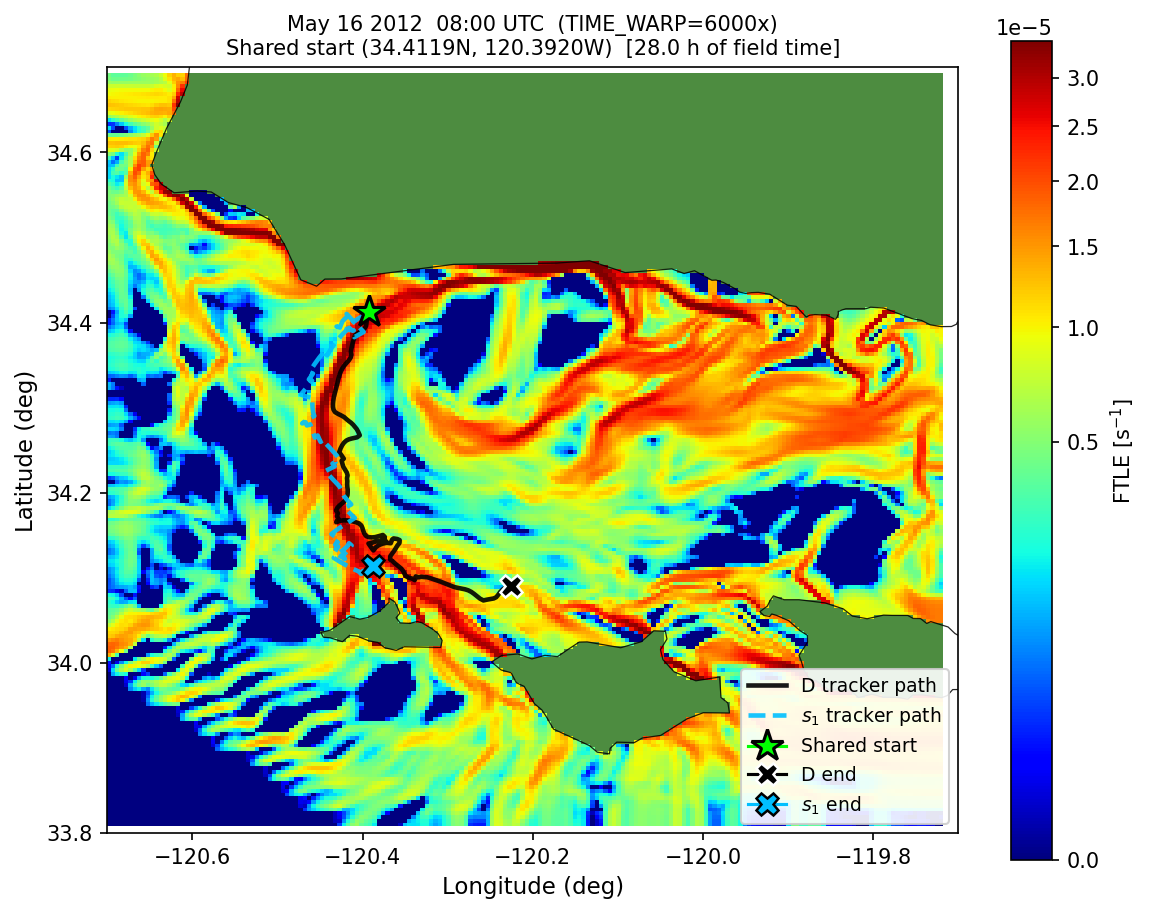
\includegraphics[width=0.38\textwidth]{figures/ocean_ftle_trajectory_overlay_2km.png}
    \caption{28-h $D$ and $s_1$ tracker paths, from a single shared
    start, over the 24-h forward FTLE field computed offline from the
    same 2~km data, anchored at the record start. Both paths follow the dominant ridge from the
    channel entrance to the bifurcation and separate only near
    landfall, where the $D$ tracker reaches the middle island's north
    coast and the $s_1$ tracker is still converging on the same target
    when the 28-h record ends.}
    \label{fig:ocean_ftle}
\end{figure}

The ocean record removes the coincidence Section~\ref{sec:disc_clean} rests
on. A measured field has no reason to carry a vorticity-free trench
network, so (\ref{eq:trench_coincide}) no longer forces the two surrogates
onto a common curve. The measured field carries a nonzero horizontal
divergence, and along the tracking corridor the exact discrepancy of
Section~\ref{sec:strain_field}, $2|\mu|/r$, has median $0.8$--$1.1$ and
90th percentile $3.0$--$5.9$ across the two primitives' paths: comparable
to the deviatoric strain rather than small, so the $s_2 = -s_1$
substitution of (\ref{eq:splitting}) is not tightly bounded here and the
splitting-identity reading of the two primitives' agreement is qualified
accordingly on this field. Both were run unmodified from a single shared
start north of the channel entrance,
$(34.41^{\circ}\mathrm{N}, -120.39^{\circ}\mathrm{W})$, at the operating
point given above, and evaluated against the 24-h forward-time FTLE
field anchored at the record start, computed offline from the full radar
grid. The $s_1$ tracker's depth condition
latched at the very first step and stayed latched for the entire
168-step run, so the ride, not gradient descent on an unlatched field, is
what the record reports. Both primitives spend the record near the edge
of their command authority rather than inside it: the $s_1$ tracker
realizes a mean centroid speed of 0.772~m/s, 89\% of the
$\sqrt{2}\,k\,c_{\max}$ cap, with its transverse channel saturated on
98.8\% of steps, and the $D$ tracker reaches that cap exactly at
0.87~m/s peak against a 0.71~m/s mean. The formation
stays far from the conic degeneracy of Remark~\ref{rem:conic} for both
primitives, at $\kappa(\boldsymbol{\Phi}) = 688$ throughout the corridor
and RMS deviation from the nominal pairwise distances under $10^{-9}$,
so the conditioning limit of Section~\ref{sec:estimation} is never
approached on this field.
Over the 28~h trial both descend through
the channel entrance and track the same ridge through the bifurcation,
their paths overlapping for nearly the entire record, and they separate
only in the final stretch, where the $D$ tracker continues to landfall on
the middle island's north coast while the $s_1$ tracker is still closing on
the same target when the budget ends.

What survives the loss of pointwise agreement is the corridor.
Fig.~\ref{fig:ocean_ftle} places both trials against the 24-h forward-time
FTLE field, computed offline over the same window in the style of
\cite{15}. Both follow the dominant ridge from the channel entrance to the
bifurcation closely: mean distance from the tracked path to the nearest
95th-percentile ridge point is 1.8~km for the $D$ tracker and 2.4~km for
the $s_1$ tracker (max 6.0 and 7.1~km), against the 2~km grid and the
5.4~km formation radius, without that ridge being available to either
primitive at any point, since only the local estimates built from the
current samples at the formation enter the commands. Forward FTLE
recomputed at four anchor times across the record (0, 5, 10, and 16~h,
each integrated 12~h forward, the longest horizon the 29-frame record
supports at four anchors) confirms that the dominant ridge
persists while the finer structure downstream evolves, and the $D$
tracker's outcome is not knife-edge sensitive to the start, with 84 of 100
jittered starts on a $10 \times 10$ grid landing on the same
middle-island branch. Two primitives reading different halves of the
same splitting identity, from a shared start on a measured field, agree
on which corridor the transport skeleton occupies while disagreeing
about the trajectory inside it.

Instantaneous criteria of this kind are not in general reliable indicators
of the material transport skeleton \cite{23}. The double gyre is a
favorable special case, and this is a finding on one record rather than a
guarantee that carries to arbitrary flows. The record is also genuinely
time-varying, with each primitive seeing only the instantaneous samples at
its own formation position and no analytic guarantee offered for that case.

The field is generic in a second way that matters for the $s_1$ tracker. It
has isolated degeneracies and cores that move between frames, so the
trial exercises tangent selection (\ref{eq:tangent_select}) where
neither the eigenframe nor the trench network is axis-aligned, which the
double gyre cannot do. It offers no genuine two-dimensional minimum of
$s_1$ within reach of the ride, so the reachability condition of Problem 2
does not engage, (\ref{eq:capture_test}) never fires, and the same
unmodified primitive behaves as a traverser. Which of the two behaviors
appears, capture on the double gyre and traverse on the ocean, is a
property of the field and not of a setting, since the terminal test is
unconditional by design and has no mode to select.

\subsection{Limitations}
\label{sec:limitations}

The scope of the underlying framework should be stated plainly. Cluster
space control is centralized, requires global state, becomes intractable
for suitably large clusters, and is impractical without reliable
high-bandwidth communication among the robots \cite{36}. The claims here
are therefore made for small clusters operating in a limited workspace
with ample bandwidth, which is the regime the six-robot estimator of
Section~\ref{sec:estimation} occupies by construction.

Within that regime, four limitations bear on the primitives. First, the
fit is ill-conditioned whenever the six sampling
points drift toward a common conic (Remark~\ref{rem:conic}). No field
tested here drives the formation toward one
(Section~\ref{sec:disc_ocean}), so the estimator is untested in the
regime its own conditioning limit describes, and the direct mitigation,
monitoring $\kappa(\boldsymbol{\Phi})$ and adding a shape-maintenance
term, is not implemented.
Second, noise can chatter the $D$ tracker across the band boundary
(\ref{eq:flow_band}), which costs only along-trench speed, since both
branches of (\ref{eq:vpar}) share the same transverse dynamics. Third,
the strain eigenframe is fragile where $\mathbf{S}$ approaches isotropy,
the $1/r$ exposure of Section~\ref{sec:sensitivity}. Tangent selection
(\ref{eq:tangent_select}) is the defense once the ride is underway, and
the residual risk of a wrong branch at a crossing under heavy noise is
damped but not excluded by the latch on (\ref{eq:capture_test}).

Fourth, and sharpest, is the $s_1$ tracker's tangent rule. Its exposure
is the eigenvector comparison rather than the seed
(Section~\ref{sec:disc_noise}), so remedies aimed at the seed do not
reach it. Holding the tangent whenever the argmax margin
$\bigl||\nabla\hat{s}_1^\top\mathbf{e}_1| -
|\nabla\hat{s}_1^\top\mathbf{e}_2|\bigr|$ falls below the noise floor
$\gamma_2\sigma_{\mathrm{eff}}/\rho^2$ of (\ref{eq:gain_ladder}) refuses
the decision instead of taking it at chance, costs no objectivity, and
is now implemented and swept on
the single-far-saddle acquisition trial (10\,000 trials/cell): success
rises from 44.6\% to 84.1\% at $\sigma_{uv} = 0.002$ and 6.0\% to
50.0\% at 0.003, narrowing above $\sigma_{uv} = 0.005$ where holding the
tangent longer starts costing along-trench progress. Two further,
unimplemented changes remain: re-running the sign decision against the
flow whenever the selected axis changes, and, for a cluster with a
trusted heading, resolving the sign against a world axis every step.

No controlled head-to-head against the straddle family \cite{17,18,19} or
the onboard-FTLE strategy of \cite{21} was run: running those methods
from an off-structure start is outside their own stated problems, and
their robots are advected (eq.~1a in \cite{17}, eq.~5a in \cite{21})
while this paper's are not (Section~\ref{sec:problem_statement}), so
one simulator cannot host both without altering one of them. All
results are from simulation; the no-advection premise is exact for the
planned Decabot hardware follow-on, where the field is encoded and read
rather than physically experienced \cite{39}, but on the ocean field it
is an extrapolation, untested against real advection.

\section{Conclusion}
\label{sec:conclusion}

This paper has presented two adaptive navigation primitives that track
the instantaneous coherent structures of a planar flow with a
six-robot cluster, using only synchronous local velocity measurements,
with no map, no forecast, no integration horizon, and no assumption
about the structure's identity. A cooperative estimator recovers the
local quadratic model of the field from one sample, six robots being
the minimum for the unconstrained model
(Proposition~\ref{prop:minimality}), with noise gains verified to
within 2.1\%. The fit supplies both terms of the splitting identity
$D = \omega^2/4 - s_1^2$, and each primitive reads one of them: the
$D$ tracker a modified Newton step on the determinant, the $s_1$
tracker a projected gradient descent on the objective strain
eigenvalue with a terminal test built only from that gradient. The
layered architecture is what makes the pair interchangeable. Both
primitives read the same fit and present the same interface to the
cluster space layer beneath them, so switching surrogates costs one
function call rather than a new estimator, a new formation, or a new
controller.

Read together, the four experiment families give an operational
selection rule. On a clean field in an inertial frame the two
primitives are interchangeable, and (\ref{eq:trench_coincide}) states
when that holds exactly. With a noisy sensor the $D$ tracker holds a
full grid step longer and fails by decay rather than by inversion; its
ceiling is set by the estimator, its failure cliff falling within 5\%
of the noise level at which $\nabla\hat{D}$ stops being informative,
while the $s_1$ tracker's ceiling is set earlier and by its own law,
in an eigenvector comparison that weighs a coefficient whose true
value is zero on the structure against one that vanishes where the
ride ends. Under a rotating observer the ranking reverses: the $D$
tracker does not degrade but leaves the structure entirely, final gap
1.219, while the $s_1$ tracker returns the same material curve in both
frames, final gap 0.025. On real Santa Barbara Channel currents both
followed the same dominant transport corridor for 28 hours, within
1.8 and 2.4~km of an FTLE ridge neither could see. The operator's
choice therefore depends on the observing platform rather than on the
flow: a cluster that can certify its orientation against a trusted
external reference should carry the $D$ tracker, which tolerates a
noisier sensor; a cluster that cannot should carry the $s_1$ tracker,
which alone returns the same material curve regardless of frame.

The primitives are admittedly simple, reactive, and minimal in robot
count, and they consume instantaneous information with no temporal
filtering whatsoever. Without question, performance and robustness can
be improved with additional robots, filtering across control cycles,
and more sophisticated control laws. Even in their present form,
however, they demonstrate acquisition from off-structure starts,
traversal through saddle points and isotropic points, terminal capture
where the field supports it, and corridor tracking on a measured
record, which is the suite of behaviors a structure-tracking mission
requires.

Ongoing and future work is targeted at a) extending the stability
results to time-varying fields with a feedforward time-derivative term
and a quantified bound, b) online formation reshaping to protect the
conditioning of $\boldsymbol{\Phi}$, including ring rotation within a
run to average out the orientation-dependent truncation bias that sets
the zero-noise tracking error, c) verifying and validating both
primitives experimentally on the Decabot testbed and thereafter in
field applications with surface vessels, d) extending the techniques
to three-dimensional fields, which raises the estimation problem to
ten coefficients per component, e) broadening the catalog of tracked
features beyond critical points to transient attracting profiles and
eddy cores, and so on.

\appendices

\section{Stability Properties}
\label{app:stability}

The analysis is at the navigation level, with the cluster centroid a
kinematic integrator
\begin{equation}
    \dot{\mathbf{p}}_c = k\,\boldsymbol{\delta}(\mathbf{p}_c),
    \label{eq:kinematic_model}
\end{equation}
$\boldsymbol{\delta}$ the right-hand side of the active law,
(\ref{eq:d_law}) or (\ref{eq:oecs_law}), and $k > 0$ the navigation
gain. The layers beneath settle in roughly 0.3~s against transit times
of tens of seconds \cite{9}. Estimates are taken exact, so hats are
dropped.

Let $\Sigma$ be the tracked surrogate, $D$ or $s_1$, in arclength
coordinates $(\ell, n)$ along and across a trench segment $\Gamma$ on a
tube $T_w = \{|n| \leq w\}$, where
\begin{equation}
    \Sigma(\ell, n) = h(\ell)
        + \tfrac{1}{2}\kappa_\perp(\ell)\,n^2,
    \qquad 0 < \underline{\kappa} \leq \kappa_\perp(\ell),
    \label{eq:normal_form}
\end{equation}
with vanishing cross terms. The lower bound $\underline{\kappa} > 0$ is
a real restriction on where $\Gamma$ may run, and it is the $s_1$
tracker that pays it. For $\Sigma = s_1$ on the double gyre,
(\ref{eq:s1_analytic_main}) gives $\kappa_{\perp} = \pi^4 A
\lvert\cos \pi y_f\rvert$ along the separatrix, which is zero at
$y = 0$, the isotropic point of $\mathbf{S}$ (Table~\ref{tab:bandwidth}
prints $a_{\perp,s_1} = 0$ there). For $\Sigma = D$ the same segment
carries $\kappa_\perp = 2\pi^6 A^2$, constant and positive, so the $D$
law is unaffected. Accordingly $\Gamma$ is taken to omit a ball
$B_\epsilon$ of radius $\epsilon$ about each isotropic point of
$\mathbf{S}$, and Lemma~\ref{lem:transit} covers the omitted arcs.
$\Gamma$ is taken invariant under the flow,
with $\lVert\mathbf{v}\rVert \geq f_{\min} > 0$ outside balls of radius
$r_0$ around the flow saddles, and $|h'(\ell)| \geq m_h > 0$ wherever
the band test fails on $\Gamma$. The transverse gradient $\kappa_\perp
n$ vanishes on $\Gamma$ and nowhere else in the tube, so the problem
splits, regulate $n$ to zero and transport along $\ell$.

Both primitives command the same transverse law
\begin{equation}
    \dot{n} = -k\,c_{\max}\tanh\!\left(
        \frac{a_\perp\,n}{c_{\max}}\right),
    \label{eq:n_dynamics}
\end{equation}
and differ only in the transverse rate $a_\perp$. The $D$ tracker
normalizes by the estimated curvature, so $a_{\perp,D} = \kappa_\perp /
\hat{\kappa}_\perp$, which is unity when the fit returns the field's
transverse curvature and is otherwise the ratio between them. The
Newton argument $-\kappa_\perp n/\kappa_\perp = -n$ therefore holds only
where the floor $e_H$ of Section~\ref{sec:sensitivity} vanishes, which on
the benchmark is the crest alone. The $s_1$ tracker has no usable curvature to normalize by
(Remark~\ref{rem:s1hess}), so its rate is set by the field,
$a_{\perp,s_1} = g_\perp\,\kappa_\perp(\ell)$.
With $V = \tfrac{1}{2}n^2$, $\dot{V} = -k\,c_{\max}\,n\tanh(a_\perp
n/c_{\max}) < 0$ for $n \neq 0$, so $T_w$ is forward invariant, the
proportional region $|n| < c_{\max}/a_\perp$ is entered in finite time,
and inside it $\dot{V} \leq -2k\,a_\perp\tanh(1)V$.

\begin{theorem}[Network traversal]
\label{thm:separatrix}
Under (\ref{eq:normal_form}) and the flow conditions above, with exact
estimates, every
trajectory of either law starting in $T_w$ (i) remains in $T_w$, converges
in finite time to the proportional band, and exponentially thereafter to $\Gamma$, and (ii) traverses $\Gamma$ in the direction
of the ambient flow, reaching the $r_0$ neighborhood of a flow saddle in
finite time bounded by $L_\Gamma/(k\,m)$, with $L_\Gamma$ the length of
$\Gamma$ and $m > 0$ the realized tangential speed.
\end{theorem}

The theorem's hypothesis holds for the class of fields on which the
relevant curvature stays indefinite along $\Gamma$. The double gyre is
not in that class for the $D$ law over the outer half of each separatrix
segment ($|y| > 0.25$), where the true $\mathbf{H}_D$ is positive
definite and the guard would fire under exact estimates
(Section~\ref{sec:sep_controller}). The fitted law's traversal there is
carried instead by the finite-radius truncation bias of
Section~\ref{sec:sensitivity} making $\hat{\mathbf{H}}_D$ traceless and
therefore artificially indefinite.

\begin{IEEEproof}
Part (i) is the transverse argument above, which holds in both branches
of (\ref{eq:vpar}) since neither transverse command contains $v_\parallel$, the
exponential rate following from concavity of $\tanh$, and holds for
(\ref{eq:oecs_law}) because $\mathbf{P}$ removes the along-trench
component of $\nabla s_1$ at $\beta = 1$, leaving the transverse channel
already treated at (\ref{eq:n_dynamics}) with $a_{\perp,s_1} =
g_\perp\kappa_\perp$. For (ii), the $s_1$ tracker commands a constant tangential speed $c_{\max}\tanh(1)$ with direction fixed by the ambient flow seed, satisfying the claim identically. On the $D$ law, both
branches return $v_\parallel \geq 0$ with $\mathbf{w}_1$ signed so that
$\hat{\mathbf{v}}_0^\top\mathbf{w}_1 \geq 0$, and each is bounded below,
by $f_{\min}$ on the band and by $m_h/\bar{\lambda}_\parallel$ off it,
with $\bar{\lambda}_\parallel$ bounding $|\lambda_1|$ on the tube. Since
$\tanh$ is increasing, the realized tangential speed is at least
\begin{equation}
    m = c_{\max}\min\bigl\{\tanh(f_{\min}/c_{\max}),\;
    \tanh(m_h/\bar{\lambda}_\parallel c_{\max})\bigr\},
    \label{eq:m_bound}
\end{equation}
and (i) holds in both branches, so the band test cannot reverse $\ell$
and a trench of length $L_\Gamma$ takes at most $L_\Gamma/(k\,m)$, the kinematic model (\ref{eq:kinematic_model}) realizing position rate $k$ times the commanded speed. On the
$s_1$ law the tangential channel of (\ref{eq:oecs_law}) is
$\beta c_{\max}\tanh(1)\mathbf{t}$ with $\beta = 1$ and
$\lVert\mathbf{t}\rVert = 1$ throughout the ride; the $\tanh(1)$ factor
is simply the saturation of a unit command, the same
$c_{\max}\tanh(c/c_{\max})$ every channel passes through, evaluated at
$c = c_{\max}$. So the realized
tangential speed is $c_{\max}\tanh(1)$ identically, in the units of
(\ref{eq:m_bound}), and $m > 0$ follows without an infimum having to be
constructed. Its direction is fixed once, at first contact, by the seed
$\mathbf{t}_{\mathrm{ref}} = \hat{\mathbf{v}}_0$ of
(\ref{eq:tangent_select}), which is the ambient flow direction, and is
propagated by the continuity factor there, which returns
$\mathbf{t}^\top\mathbf{t}_{\mathrm{ref}} =
\lvert\mathbf{t}_{\mathrm{raw}}^\top\mathbf{t}_{\mathrm{ref}}\rvert
\geq 0$ and so cannot reverse $\ell$ in one step. With exact estimates
the argmax in (\ref{eq:tangent_select}) returns the along-trench
eigenvector at every point of $\Gamma$ where $\nabla s_1 \neq 0$, so the
seeded direction persists along the segment.
\end{IEEEproof}

The direction claim in (ii) rests on the exact-estimate hypothesis for
both laws. Once the estimates carry noise, the argmax rather than the
seed decides the $s_1$ tracker's tangent, and the traversal direction can
invert.

The primitives end differently at a saddle. There $D$ has a local
minimum with $\mathbf{H}_D \succ 0$ and the degenerate case of
(\ref{eq:d_law}) is active, but the floor $e_H$ of
Section~\ref{sec:sensitivity} leaves the estimated eigenvalues
indefinite even without noise, so the $D$ tracker rides onto the
crossing segment and repeats (i) and (ii) with $\Gamma$ relabeled. The
$s_1$ tracker stops. Once the ride flag clears, the projector is the
identity, (\ref{eq:oecs_law}) is gradient descent on the surrogate
itself, and $\dot{s}_1 \leq 0$ with equality only at a critical point.
That is the vanishing-gradient test Section~\ref{sec:sensitivity} admits
rather than the definiteness test it does not.

Estimation error, and any residual cross term $\kappa_\perp'(\ell)\,n$,
enters the transverse channel as a bounded disturbance $|d| \leq
\delta$. Then $\dot{V} < 0$ outside an interval and the structure is
practically stable, with
\begin{equation}
    \limsup_{t\to\infty}|n(t)| \;\leq\;
    \frac{c_{\max}}{a_\perp}
    \operatorname{artanh}\!\left(\frac{\delta}{k\,c_{\max}}\right)
    \;\approx\; \frac{\delta}{k\,a_\perp},
    \label{eq:iss_bound}
\end{equation}
provided the disturbance is strictly bounded by the actuator authority, $\delta < k\,c_{\max}$. Two disturbances enter here and they behave
differently. The zero-mean part is the noise on the transverse gradient,
placed at $\nu/\tilde{\rho}^{\,2}$ by (\ref{eq:error_budget}), which
makes tracking error degrade linearly in measurement noise. The
orientation-dependent truncation bias of
Section~\ref{sec:sensitivity} is not zero mean and does not vanish on
$\Gamma$, so it displaces the equilibrium of
(\ref{eq:n_dynamics}) rather than spreading it. Its size is the
displacement between the fitted trench and the field's, and it is
independent of $k$ and of the saturation.

Neither (\ref{eq:n_dynamics}) nor (\ref{eq:iss_bound}) survives at an
isotropic point, where $a_{\perp,s_1} = g_\perp\kappa_\perp$ vanishes and
(\ref{eq:iss_bound}) divides by it. The excluded arcs are covered
separately, and what carries the cluster across them is the ride.

\begin{lemma}[Isotropic transit]
\label{lem:transit}
Let $\mathbf{p}^\circ$ be an isotropic point of $\mathbf{S}$ on the
tracked network and $B_\epsilon$ the ball of radius $\epsilon$ about it
excluded from $\Gamma$. Suppose the $s_1$ tracker enters $B_\epsilon$
with $|n| \leq n_0$, its ride flag latched, under the same bounded
disturbance $|d| \leq \delta$. Then it leaves $B_\epsilon$ within
transit time
\begin{equation}
    T_\epsilon \;\leq\; \frac{2\epsilon}{k\,c_{\max}\tanh(1)},
    \label{eq:transit_time}
\end{equation}
and throughout the transit
\begin{equation}
    |n(t)| \;\leq\; n_0 + \delta\,T_\epsilon
    \;=\; n_0 + \frac{2\epsilon\,\delta}{k\,c_{\max}\tanh(1)}
    \;=\; n_0 + O(\epsilon).
    \label{eq:transit_growth}
\end{equation}
\end{lemma}

\begin{IEEEproof}
The tangential channel of (\ref{eq:oecs_law}) is
$\beta c_{\max}\tanh(1)\mathbf{t}$ with $\beta = 1$ and
$\lVert\mathbf{t}\rVert = 1$, and it contains no curvature, so it is
unchanged as $\kappa_\perp \to 0$. The kinematic model
(\ref{eq:kinematic_model}) then realizes position rate
$k\,c_{\max}\tanh(1)$ along $\Gamma$, and a chord of $B_\epsilon$ has
length at most $2\epsilon$, giving (\ref{eq:transit_time}).
For the transverse channel, (\ref{eq:n_dynamics}) holds for every
$a_\perp \geq 0$, and since $\tanh$ is odd and increasing,
$n\tanh(a_\perp n/c_{\max}) \geq 0$, so the restoring term is
non-positive in $\tfrac{d}{dt}\tfrac{1}{2}n^2$ at every $a_\perp$,
degenerating to no contribution at $a_\perp = 0$ rather than changing
sign. Hence $\tfrac{d}{dt}|n| \leq \delta$ inside $B_\epsilon$, and
integrating over $T_\epsilon$ gives (\ref{eq:transit_growth}).
\end{IEEEproof}

The isotropic point removes the transverse restoring force, but it
removes the transverse gradient with it, so nothing steers the cluster
off the structure while it crosses and the ride carries it through at
constant speed. Transit is $O(\epsilon)$ and the error it admits is
$O(\epsilon)$ with it, so a trajectory leaving $B_\epsilon$ re-enters
Theorem~\ref{thm:separatrix}'s hypotheses with an initial condition
still inside $T_w$ for $\epsilon$ small enough, and the exponential
argument resumes on the next segment. At $\delta = 0$ the bound
conserves $|n|$ exactly, which is the noise-free crossing
Section~\ref{sec:disc_clean} reports at the origin.

A bandwidth limit sits underneath this, and the actuator changes it.
Explicit Euler on (\ref{eq:kinematic_model}) alone would make the
near-structure map $n \mapsto n(1 - \Delta t\,k\,a_\perp)$, monotone
below $\Delta t\,k\,a_\perp = 1$ and stable below $2$. Closing
(\ref{eq:momentum}) around $-k\,a_\perp n$ instead gives a two-state map
of determinant $\alpha_{\text{mom}}$ for every gain, so where its
eigenvalues are complex the transverse error decays at
$\sqrt{\alpha_{\text{mom}}}$ per step irrespective of $a_\perp$. With
$\beta = \Delta t\,k\,a_\perp(1 - \alpha_{\text{mom}})$ the spectrum is
real and positive below $\beta = (1 - \sqrt{\alpha_{\text{mom}}})^2$,
complex with modulus $\sqrt{\alpha_{\text{mom}}}$ between that value and
$(1 + \sqrt{\alpha_{\text{mom}}})^2$, real negative between
$(1 + \sqrt{\alpha_{\text{mom}}})^2$ and $2(1 + \alpha_{\text{mom}})$, and
unstable above $\beta = 2(1 + \alpha_{\text{mom}})$. The lag the
kinematic abstraction treats as a separate limit is what relaxes the
discrete one, so the two cannot be read independently.
Table~\ref{tab:bandwidth} evaluates both bounds at the double-gyre
operating point.

\begin{table}[!t]
\centering
\caption{Transverse rate of each law along a separatrix segment, and the
fraction of that segment past the discrete bounds of this appendix,
at the double-gyre operating point
($\Delta t = 0.1$, $k = 3.0$,
$\alpha_{\text{mom}} = 0.7$, $g_\perp = 1.0$). Neither $a_\perp$ is a
constant. The $D$ tracker's follows from
(\ref{eq:floor_closed}) and the $s_1$ tracker's from
(\ref{eq:s1_analytic_main}), both in closed form. The last column uses
the bound that accounts for the actuator, $\Delta t\,k\,a_\perp
(1-\alpha_{\text{mom}}) > 2(1+\alpha_{\text{mom}})$, which here is
$\Delta t\,k\,a_\perp > 11.3$, and evaluates $a_{\perp,D}$ on the
realized fit rather than on exact estimates.}
\label{tab:bandwidth}
\footnotesize
\setlength{\tabcolsep}{3pt}
\begin{tabular}{@{}lccccccc@{}}
\hline
 & $a_\perp(y)$ & \multicolumn{3}{c}{$\Delta t\,k\,a_\perp$ at}
 & \multicolumn{2}{c}{fraction past} \\
\cline{3-5}\cline{6-7}
 & & $y\!=\!0$ & $|y|\!=\!0.35$ & $|y|\!\to\!0.5$
 & $\Delta t k a_\perp\!=\!1$ & instab. \\
\hline
$D$ & $\csc^2 \pi y_f$ & $0.30$ & $1.46$ & $\infty$ & 36.8\% & 10.4\% \\
$s_1$ & $g_\perp \pi^4 A |\cos \pi y_f|$ & $0$ & $2.60$ & $2.92$ & 77.7\% & 0\% \\
\hline
\end{tabular}
\end{table}

\section{Frame Equivariance of the $s_1$ Tracker}
\label{app:equivariance}

\begin{proposition}[Frame equivariance of the closed loop]
\label{prop:equivariance}
Let an observer rotate as $\mathbf{p}_Q = \mathbf{Q}(t)\mathbf{p}$ and
let the $s_1$ tracker run with exact estimates on the correspondingly
transformed field. Then the command is equivariant,
$\boldsymbol{\delta}_Q = \mathbf{Q}\boldsymbol{\delta}$. If in addition
the frame-transport speed is dominated by the command authority on the
tube,
\begin{equation}
    \Omega\,\lVert\mathbf{p}_Q\rVert \;<\; k\,c_{\max} ,
    \label{eq:transport_cond}
\end{equation}
the path is equivariant to a bounded residue, with
$\mathbf{p}_{c,Q}(t)$ tracking $\mathbf{Q}(t)\mathbf{p}_c(t)$ at a
transverse error obeying
(\ref{eq:iss_bound}) at $\delta = \Omega\lVert\mathbf{p}_Q\rVert$, so the
tracker follows the same material structure in every frame. The single
exception is the degenerate guard, reachable only on the first tracking
step. That same first step carries a second, implicit hypothesis: the
one-time seed $\mathbf{t}_{\text{ref}} = \hat{\mathbf{v}}_0$ at first
contact is itself frame-dependent, and unlike the guard it is always
consulted, so the bounded-residue claim additionally requires the seed's
resolved sign to agree across frames. What the frame adds to the seed is
the transport velocity $\dot{\mathbf{Q}}\mathbf{Q}^\top\mathbf{p}$, and
what decides the sign is the projection on
$\mathbf{t}_{\text{raw}}$, so the condition is a comparison of
projections,
\begin{equation}
    \lvert(\dot{\mathbf{Q}}\mathbf{Q}^\top\mathbf{p}_{\text{seed}})^\top
    \mathbf{t}_{\text{raw}}\rvert
    \;<\; \lvert\hat{\mathbf{v}}_0^\top\mathbf{t}_{\text{raw}}\rvert,
    \label{eq:seed_cond}
\end{equation}
at the seed point $\mathbf{p}_{\text{seed}}$; if it fails the two paths
are not close, they commit to opposite branches. Bounding the left side
by $\Omega\lVert\mathbf{p}_{\text{seed}}\rVert$ gives the sufficient
corollary
\begin{equation}
    \Omega\,\lVert\mathbf{p}_{\text{seed}}\rVert
    \;<\; \lvert\hat{\mathbf{v}}_0^\top\mathbf{t}_{\text{raw}}\rvert,
    \label{eq:seed_cond_suff}
\end{equation}
which is the version a cluster can check without resolving the tangent
first.
\end{proposition}

\begin{IEEEproof}
By Section~\ref{sec:strain_field} the transport term in $\mathbf{J}_Q$ lands in the
spin part, so $\mathbf{S}_Q = \mathbf{Q}\mathbf{S}\mathbf{Q}^\top$,
leaving $s_1$ and $r$ invariant and the eigenframe and $\nabla s_1$
co-rotating. Every test in (\ref{eq:oecs_law}) and
(\ref{eq:tangent_select}) is a scalar inequality in those invariants, so
the tangent is equivariant by induction from the second tracking step
onward and $\boldsymbol{\delta}_Q = \mathbf{Q}\boldsymbol{\delta}$
follows. Integration is a separate matter. The rotating frame gives
$\dot{\mathbf{p}}_Q = k\boldsymbol{\delta}_Q$ while the transported
inertial path satisfies $\tfrac{d}{dt}(\mathbf{Q}\mathbf{p}_c) =
k\mathbf{Q}\boldsymbol{\delta} +
\dot{\mathbf{Q}}\mathbf{Q}^\top\mathbf{p}_Q$, so an equivariant command
integrated in a rotating frame is not itself path equivariant, the two
differing by the transport velocity $\Omega\lVert\mathbf{p}_Q\rVert$.
Its transverse component is a bounded disturbance on
(\ref{eq:n_dynamics}), so under (\ref{eq:transport_cond}) the
practical-stability argument of (\ref{eq:iss_bound}) bounds the residue
rather than letting it accumulate. The degenerate guard is the exception.
It reads the
measured flow, carrying
$\dot{\mathbf{Q}}\mathbf{Q}^\top\mathbf{p}_Q$ with no inertial
counterpart, and is reachable only on the first tracking step, before
continuity takes over. The same first step is where
(\ref{eq:seed_cond}) is tested. At the objectivity trial's start
$(0.05, 0.40)$ with $\Omega = 0.2$ the shear strain vanishes
identically, so the eigenvectors are the coordinate axes and the argmax
of (\ref{eq:tangent_select}) returns $\mathbf{t}_{\text{raw}} =
\hat{\mathbf{e}}_y$ ($\lvert\nabla s_1 \cdot \hat{\mathbf{e}}_y\rvert =
0.946$ against $0.461$ for $\hat{\mathbf{e}}_x$), giving
$\lvert\hat{\mathbf{v}}_0^\top\mathbf{t}_{\text{raw}}\rvert = 0.096$.
The transport velocity is
$\dot{\mathbf{Q}}\mathbf{Q}^\top\mathbf{p}_{\text{seed}} = \Omega(-y,
x)^\top = (-0.080, 0.010)^\top$, nearly orthogonal to
$\mathbf{t}_{\text{raw}}$, so the left side of (\ref{eq:seed_cond}) is
$0.010$ and the margin is $9.6\times$; the critical rate is
$\Omega \approx 1.92$, an order of magnitude above the rate run. The
sufficient form (\ref{eq:seed_cond_suff}) is much more conservative at
the same point, $\Omega\lVert\mathbf{p}_{\text{seed}}\rVert = 0.081$
against the same $0.096$, a margin of $1.19\times$ and a critical rate
of $\Omega \approx 0.238$.
\end{IEEEproof}

The $D$ tracker admits no counterpart, since its surrogate carries the
additive frame term $\Omega\omega + \Omega^2$ of
(\ref{eq:D_not_objective}) into everything its law reads. That term is
absolute rather than relative. Measured against $D$ itself it is
unbounded wherever $D$ vanishes, and $D$ vanishes at the crest the
primitive is required to cross.

\begin{thebibliography}{99}
\bibitem{1} J. Cortés and M. Egerstedt, ``Coordinated control of multi-robot
systems: A survey,'' \textit{SICE Journal of Control, Measurement, and
System Integration}, vol. 10, no. 6, pp. 495--503, 2017.

\bibitem{2} P. Ögren, E. Fiorelli, and N. E. Leonard, ``Cooperative control
of mobile sensor networks: Adaptive gradient climbing in a distributed
environment,'' \textit{IEEE Transactions on Automatic Control}, vol. 49, no. 8,
pp. 1292--1302, 2004.

\bibitem{3} R. T. McDonald, C. A. Kitts, and M. A. Neumann, ``Navigation of
scalar fronts with multirobot clusters in simulation and experiment,''
\textit{IEEE Systems Journal}, vol. 14, no. 3, pp. 3755--3766, 2020.

\bibitem{4} C. A. Kitts, R. T. McDonald, and M. A. Neumann, ``Adaptive
navigation control primitives for multirobot clusters: Extrema finding,
contour following, ridge/trench following, and saddle point station keeping,''
\textit{IEEE Access}, vol. 6, pp. 17625--17642, 2018.

\bibitem{5} R. T. McDonald, C. A. Kitts, and M. A. Neumann, ``Experimental
implementation and verification of scalar field ridge, trench, and saddle
point maneuvers using multirobot adaptive navigation,'' \textit{IEEE Access},
vol. 7, pp. 62950--62961, 2019.

\bibitem{6} L. Briñón-Arranz, A. Renzaglia, and L. Schenato, ``Multirobot
symmetric formations for gradient and Hessian estimation with application to
source seeking,'' \textit{IEEE Transactions on Robotics}, vol. 35, no. 3,
pp. 782--789, 2019.

\bibitem{7} M. Mateus, R. Canelas, L. Pinto, and N. Vaz, ``When
tragedy strikes: Potential contributions from ocean observation to
search and rescue operations after drowning accidents,'' \textit{Front.
Mar. Sci.}, vol. 7, art. 55, 2020.

\bibitem{8} P. Keramea, K. Spanoudaki, G. Zodiatis, G. Gikas, and
G. Sylaios, ``Oil spill modeling: A critical review on current trends,
downscaling, and applications,'' \textit{J. Mar. Sci. Eng.}, vol. 9,
no. 2, art. 181, 2021.

\bibitem{9} C. Waight and C. A. Kitts, ``Adaptive navigation of multirobot
systems to critical points in 2D vector fields,'' submitted for publication.

\bibitem{10} J. Das, F. Py, T. Maughan, T. O'Reilly, M. Messié, J. Ryan,
G. S. Sukhatme, and K. Rajan, ``Coordinated sampling of dynamic oceanographic
features with underwater vehicles and drifters,'' \textit{The International
Journal of Robotics Research}, vol. 31, no. 5, pp. 626--646, 2012.

\bibitem{11} S. McCammon, G. Marcon dos Santos, M. Frantz, T. P. Welch,
G. Best, R. K. Shearman, J. D. Nash, J. A. Barth, J. A. Adams, and
G. A. Hollinger, ``Ocean front detection and tracking using a
team of heterogeneous marine vehicles,'' \textit{Journal of Field Robotics},
vol. 38, no. 6, pp. 854--881, 2021.

\bibitem{12} S. R. Ramp et al., ``Preparing to predict: the second autonomous
ocean sampling network (AOSN-II) experiment in the Monterey Bay,''
\textit{Deep Sea Research Part II: Topical Studies in Oceanography}, vol. 56,
no. 3-5, pp. 68--86, 2009.

\bibitem{13} G. Haller and G. Yuan, ``Lagrangian coherent structures and mixing
in two-dimensional turbulence,'' \textit{Physica D: Nonlinear Phenomena},
vol. 147, no. 3-4, pp. 352--370, 2000.

\bibitem{14} T. Peacock and G. Haller, ``Lagrangian coherent structures: The
hidden skeleton of fluid flows,'' \textit{Physics Today}, vol. 66, no. 2,
pp. 41--47, 2013.

\bibitem{15} S. C. Shadden, F. Lekien, and J. E. Marsden, ``Definition and
properties of Lagrangian coherent structures from finite-time Lyapunov
exponents in two-dimensional aperiodic flows,'' \textit{Physica D}, vol. 212,
no. 3-4, pp. 271--304, 2005.

\bibitem{16} C. Dong et al., ``Oceanic mesoscale eddies,'' \textit{Ocean-Land-
Atmosphere Research}, vol. 4, p. 0081, 2025.

\bibitem{17} M. Michini, M. A. Hsieh, E. Forgoston, and I. B. Schwartz,
``Robotic tracking of coherent structures in flows,'' \textit{IEEE Transactions
on Robotics}, vol. 30, no. 3, pp. 593--603, 2014.

\bibitem{18} M. Michini, H. Rastgoftar, M. A. Hsieh, and S. Jayasuriya,
``Distributed formation control for collaborative tracking of manifolds in
flows,'' in \textit{Proc. American Control Conference}, pp. 3874--3880, 2014.

\bibitem{19} M. Michini, M. A. Hsieh, E. Forgoston, and I. B. Schwartz,
``Experimental validation of robotic manifold tracking in gyre-like flows,''
in \textit{Proc. IEEE/RSJ International Conference on Intelligent Robots
and Systems (IROS)}, pp. 2306--2311, 2014.

\bibitem{20} G. Knizhnik, P. Li, X. Yu, and M. A. Hsieh, ``Flow-based control
of marine robots in gyre-like environments,'' in \textit{Proc. 2022 Int. Conf.
on Robotics and Automation (ICRA)}, pp. 3047--3053, 2022.

\bibitem{21} D. Kularatne and M. A. Hsieh, ``Tracking attracting manifolds in
flows,'' \textit{Autonomous Robots}, vol. 41, no. 8, pp. 1575--1588, 2017.

\bibitem{22} R. N. Smith, M. Schwager, S. L. Smith, B. H. Jones, D. Rus,
and G. S. Sukhatme, ``Persistent ocean monitoring with underwater gliders:
Adapting sampling resolution,'' \textit{J. Field Robotics}, vol. 28, no. 5,
pp. 714--741, 2011.

\bibitem{23} G. Haller, ``Lagrangian coherent structures,'' \textit{Annual
Review of Fluid Mechanics}, vol. 47, pp. 137--162, 2015.

\bibitem{24} M. Serra and G. Haller, ``Objective Eulerian coherent
structures,'' \textit{Chaos: An Interdisciplinary Journal of Nonlinear
Science}, vol. 26, no. 5, p. 053110, 2016.

\bibitem{25} P. J. Nolan, M. Serra, and S. D. Ross, ``Finite-time Lyapunov
exponents in the instantaneous limit and material transport,''
\textit{Nonlinear Dynamics}, vol. 100, no. 4, pp. 3825--3852, 2020.

\bibitem{26} T. D. Harms, S. T. M. Dawson, and B. J. McKeon, ``Lagrangian
gradient regression for the detection of coherent structures from sparse
trajectory data,'' \textit{Royal Society Open Science}, vol. 11, no. 9,
p. 240586, 2024.

\bibitem{27} G. Haller, ``Dynamic rotation and stretch tensors from a
dynamic polar decomposition,'' \textit{Journal of the Mechanics and Physics
of Solids}, vol. 86, pp. 70--93, 2016.

\bibitem{28} A. Okubo, ``Horizontal dispersion of floatable particles in the
vicinity of velocity singularities such as convergences,'' \textit{Deep-Sea
Research}, vol. 17, no. 3, pp. 445--454, 1970.

\bibitem{29} J. Weiss, ``The dynamics of enstrophy transfer in two-dimensional
hydrodynamics,'' \textit{Physica D: Nonlinear Phenomena}, vol. 48, no. 2-3,
pp. 273--294, 1991.

\bibitem{30} J. C. R. Hunt, A. A. Wray, and P. Moin, ``Eddies, streams, and
convergence zones in turbulent flows,'' in \textit{Proc. Summer Program,
Center for Turbulence Research}, Rep. CTR-S88, pp. 193--208, 1988.

\bibitem{31} B.-L. Hua and P. Klein, ``An exact criterion for the stirring
properties of nearly two-dimensional turbulence,'' \textit{Physica D}, vol. 113,
no. 1, pp. 98--110, 1998.

\bibitem{32} R. Cooper, D. Rajabhandharaks, R. T. McDonald, M. A. Neumann,
and C. A. Kitts, ``Initial study of multirobot adaptive
navigation for exploring environmental vector fields,'' in \textit{Proc.
IEEE Aerospace Conference}, 2019.

\bibitem{33} W. Yao, H. G. de Marina, B. Lin, and M. Cao,
``Singularity-free guiding vector field for robot navigation,''
\textit{IEEE Trans. Robot.}, vol. 37, no. 4, pp. 1206--1221, 2021.

\bibitem{34} T. Liddy and T.-F. Lu, ``Obstacle avoidance using complex
vector fields,'' in \textit{Proc. Australasian Conf. Robotics and
Automation (ACRA)}, 2008.

\bibitem{35} M. Serra, P. Sathe, I. Rypina, A. Kirincich, S. D. Ross,
P. Lermusiaux, A. Allen, T. Peacock, and G. Haller, ``Search and rescue
at sea aided by hidden flow structures,'' \textit{Nature Communications},
vol. 11, no. 1, p. 2525, 2020.

\bibitem{36} C. A. Kitts and I. Mas, ``Cluster space specification and control
of mobile multirobot systems,'' \textit{IEEE/ASME Transactions on Mechatronics},
vol. 14, no. 2, pp. 207--218, 2009.

\bibitem{37} T. Adamek, C. A. Kitts, and I. Mas, ``Gradient-based cluster space
navigation for autonomous surface vessels,'' \textit{IEEE/ASME Transactions on
Mechatronics}, vol. 20, no. 2, pp. 506--518, 2014.

\bibitem{38} S. Tomer et al., ``A low-cost indoor testbed for multirobot
adaptive navigation research,'' in \textit{Proc. IEEE Aerospace Conference},
pp. 1--12, 2018.

\bibitem{39} C. Waight and C. Kitts, ``A functional indoor testbed for
multirobot adaptive navigation in vector field environments,'' in
\textit{Proc. ASME Int. Design Engineering Technical Conf. and Computers
and Information in Engineering Conf.}, vol. 89251, 2025.

\bibitem{40} NOAA National Centers for Environmental Information,
``Near-real-time surface ocean velocities derived from HF-radar stations
located along coastal waters of North Slope Alaska, Gulf of Alaska,
Puerto Rico/Virgin Islands, eastern U.S./Gulf of America, Hawaii, Great
Lakes, and western U.S.,'' NCEI Accession
gov.noaa.nodc:IOOS-HFRadarRTVector.

\end{thebibliography}

\end{document}
